\documentclass[12pt,oneside]{book} % for one-sided printing

\usepackage{blindtext}% Just used so we can generate some example text
\usepackage{amsmath}
\usepackage{algorithm}
\usepackage{algpseudocode}
\usepackage{amssymb}
\usepackage{mathtools}
\usepackage[export]{adjustbox}
\usepackage{lipsum}
\usepackage{booktabs}  % For better quality tables
\usepackage{tabularx}  % for the X column type
\usepackage{listings}
\usepackage{xcolor}
\usepackage{caption}
\usepackage{xfrac}
\usepackage{indentfirst}
\usepackage{subcaption}
\usepackage{graphicx}
\usepackage{geometry}
\geometry{a4paper, margin=1in}

% Place style file after other packages.
\usepackage{cranfieldthesis}
\usepackage{lscape} % for landscape pages
\usepackage{float}
\usepackage[toc,title,page]{appendix}

% Couleurs personnalisées
\definecolor{backcolour}{rgb}{0.96, 0.96, 0.96} % Fond très clair
\definecolor{codegray}{rgb}{0.47, 0.47, 0.47}   % Commentaires et numéros de ligne
\definecolor{codegreen}{rgb}{0.25, 0.50, 0.35}  % Commentaires
\definecolor{codeblue}{rgb}{0.26, 0.44, 0.58}   % Mots-clés
\definecolor{codepurple}{rgb}{0.50, 0, 0.50}    % Identificateurs
\definecolor{codeteal}{rgb}{0, 0.5, 0.5}        % Chaînes de caractères
\definecolor{terminalback}{rgb}{0.05, 0.05, 0.05} % Fond très sombre pour le terminal
\definecolor{terminaltext}{rgb}{0.7, 0.7, 0.7}    % Texte clair pour le terminal
\definecolor{mygreen}{rgb}{0,0.6,0}
\definecolor{mygray}{rgb}{0.5,0.5,0.5}
\definecolor{mymauve}{rgb}{0.58,0,0.82}
\definecolor{terminalbgcolor}{HTML}{330033}
\definecolor{terminalrulecolor}{HTML}{000099}

\lstdefinestyle{bashstyle}{
    language=bash,
    backgroundcolor=\color{backcolour},
    basicstyle=\ttfamily\scriptsize,
    keywordstyle=\color{blue},
    stringstyle=\color{red},
    identifierstyle=\color{codepurple},
    commentstyle=\color{codegreen},
    morecomment=[l]{\#},   % Define comment style
    frame=single,          % adds a frame around the code
    rulecolor=\color{gray},% if not set, the frame-color may be changed on line-breaks
    breakatwhitespace=false,
    breaklines=true,       % sets automatic line breaking
    captionpos=b,          % sets the caption-position to bottom
    keepspaces=true,       % keeps spaces in text
    showspaces=false,      % show spaces everywhere adding particular underscores
    showstringspaces=false % underline spaces within strings only
}

\lstdefinestyle{cstyle}{
    language=C++,
    basicstyle=\ttfamily\scriptsize,
    keywordstyle=\color{blue},
    backgroundcolor=\color{backcolour},
    stringstyle=\color{red},
    commentstyle=\color{codegreen},
    morecomment=[l][\color{magenta}]{\#},
    breaklines=true,
    numbers=left,
    numberstyle=\tiny\color{gray},
    showstringspaces=false,
    tabsize=2,
    frame=single
}

% Title Page Set Up
\title{High Performance Technical Computing Assignment}
\author{Alexis Balayre}
\date{5\textsuperscript{th} February 2024}
\school{\SATM}
\degree{MSc}
\course{Computational Software of Techniques Engineering}
\academicyear{2023 - 2024}

% Supervisors
\supervisor{Dr Irene Moulitsas}

% Copyright
\copyrightyear{2024}

% References
\usepackage[numbers]{natbib} % for nice referencing
\makeatletter % Reference list option change to number and period
\renewcommand\@biblabel[1]{#1.} % from [1] to 1
\makeatother %
\setcitestyle{round} % use round citations

\begin{document}

\frontmatter

% Form Title Pages
\maketitle

% Abstract and Keywords
\begin{abstract}
    Replace with your abstract text of not more than 300 words.
\end{abstract}

% Use single spacing for Table of Contents, List of Figures, etc
{
\clearpage
\singlespacing
% Table of Contents
{
    \tableofcontents
}
\clearpage

% List of Figures
\listoffigures

% List of Tables
\listoftables
}

%% Main Matter
\mainmatter
\pagestyle{fancy}
\fancyhead[L]{\nouppercase{\leftmark}}
\fancyhead[R]{\nouppercase{\rightmark}}

\chapter{Introduction}
High-Performance Computing (HPC) is a branch of computing that uses
supercomputers and server clusters to solve complex, computationally intensive
problems. Unlike a personal computer with a single processor, an HPC system is
made up of many processors working in parallel, considerably increasing
processing capacity. This enables scientists and engineers to carry out
detailed numerical simulations, such as forecasting the weather or solving
structural engineering problems.

Cranfield University has two HPC systems: CRESCENT2 and DELTA. However, this
report will focus exclusively on CRESCENT2, which is an HPC cluster designed to
provide computing power for teaching and research. CRESCENT 2 nodes are
equipped with Intel Xeon E5 2620 processors, and each node contains two 16-core
processors and 16 gigabytes of RAM.

The aim of this report is to explore distributed memory parallel programming
strategies for optimising the performance of sparse matrix multiplication by a
fat vector, a common operation in numerical linear algebra.

Consider a sparse matrix $M$ of dimensions $m \times n$ and a fat vector $v$ of
dimensions $n \times k$. The objective is to perform the multiplication $M
    \times v$, yielding a result that is of dimensions $m \times k$.

The matrix $M$ is defined as:
\begin{equation}
    M = \begin{pmatrix}
        m_{11} & m_{12} & \cdots & m_{1n} \\
        m_{21} & m_{22} & \cdots & m_{2n} \\
        \vdots & \vdots & \ddots & \vdots \\
        m_{m1} & m_{m2} & \cdots & m_{mn}
    \end{pmatrix}
\end{equation}\label{eq:sparse-matrix}
where most elements of $M$ are zeros.

The vector $v$ is defined as:
\begin{equation}
    v = \begin{pmatrix}
        v_{11} & v_{12} & \cdots & v_{1k} \\
        v_{21} & v_{22} & \cdots & v_{2k} \\
        \vdots & \vdots & \ddots & \vdots \\
        v_{n1} & v_{n2} & \cdots & v_{nk}
    \end{pmatrix}\label{eq:dense-vector}
\end{equation}

\chapter{Methodology}
\section{Data Structures}
In numerical computation and linear algebra, efficient use of memory and fast
computation are crucial. This is particularly true when working with hollow
matrices and fat vectors.

\subsection{Sparse Matrix}
The sparse matrix is represented in CSR (Compressed Sparse Row) format, which
is particularly effective for storing and manipulating matrices where the
majority of elements are zero. The CSR structure consists of three main
vectors:
\begin{itemize}
    \item \textbf{values}: A vector storing all the non-zero elements of the matrix.
    \item \textbf{rowPtr}: A vector storing the starting index for each element in the
          \textit{values} vector.
    \item \textbf{colIndices}: A vector storing the column indices for each element in the vector \textit{values}.
          \
\end{itemize}

Here is an example of a sparse matrix in CSR format:
\begin{itemize}
    \item \texttt{values} = \{1, 2, 3, 4\}
    \item \texttt{rowPtr} = \{0, 2, 3, 3, 4\}
    \item \texttt{colIndices} = \{0, 2, 1, 3\}
\end{itemize}

This hollow matrix can be visualised as:
\[
    \begin{bmatrix}
        1 & 0 & 2 & 0 \\
        0 & 0 & 3 & 0 \\
        0 & 0 & 0 & 0 \\
        0 & 0 & 0 & 4 \\
    \end{bmatrix}
\]

The \textbf{SparseMatrix} structure is defined in
Appendix~\ref{appendix:data-structures}.

\subsection{Fat Vector}
Unlike a hollow matrix, a fat vector (illustrated by
equation~\ref{eq:dense-vector}) stores all its elements, including zeros. The
data structure for a fat vector is a two-dimensional array, where each row
represents a separate vector. The \textbf{FatVector} structure is defined in
Appendix~\ref{appendix:data-structures}.

\section{Sequential Algorithm}
Let \( M \) be a sparse matrix of size \( m \times n \) with \( z \) non-zero
elements, stored in CSR format, and \( v \) be a fat vector of size \( n \times
k \). The sequential algorithm for multiplying \( M \) by \( v \) is
implemented in Appendix~\ref{appendix:sequential}.

\subsection{Algorithm Flow}

\begin{algorithm}[H]
    \caption{Sequential algorithm}
    \begin{algorithmic}
        \Require $M$ is an $m \times n$ sparse matrix
        \Require $v$ is an $n \times k$ fat vector
        \Ensure  $Result$ is an $m \times k$ matrix
        \State $Result \gets$ zero matrix of size $m \times k$
        \For{$i \gets 0$ \textbf{to} $m-1$}
        \For{each non-zero element $(j, \text{value})$ in row $i$ of $M$}
        \For{$j \gets 0$ \textbf{to} $k-1$}
        \State $Result[i][l] \gets Result[i][l] + (\text{value} \times v[j][l])$
        \EndFor
        \EndFor
        \EndFor
        \State \Return $Result$
    \end{algorithmic}
\end{algorithm}

The algorithmic flow can be more explicitly detailed by:
\begin{enumerate}
    \item \textbf{Initialisation:} Create a zero matrix of size \( m \times k \) to store the result.
    \item \textbf{Row-wise Processing:} Iterate over each row \(i\) of matrix \(M\), leveraging the CSR format to efficiently access non-zero elements.
    \item \textbf{Element-wise Multiplication and Accumulation:} For each non-zero element in row \(i\), identified by its column index \(j\) and value, conduct a nested iteration over the columns \(l\) of vector \(v\), multiplying the non-zero element by the corresponding vector element and accumulating the result in \(Result[i][l]\).
\end{enumerate}

\subsection{Temporal Complexity Analysis}

The time complexity can be broken down into the following components:

\begin{enumerate}
    \item \textbf{Matrix Row Traversal:} Each row of the matrix is traversed once, so the complexity of traversing all the rows is \( O(m) \).
    \item \textbf{Non-zero Element Access:} The CSR format ensures efficient access to non-zero elements, attributing a complexity of \(O(z)\) for parsing all such elements across the matrix.
    \item \textbf{Multiplication et Accumulation:} The key computational step involves multiplying each non-zero element by the corresponding entries in \(v\), across all \(k\) columns. Given that each non-zero element undergoes this operation, the complexity is more accurately described as \(O(zk)\), highlighting the direct proportionality to both the number of non-zero elements and the vector's column dimension.
\end{enumerate}

Hence, the time complexity of multiplying a sparse matrix in CSR format with a
fat matrix is \( O(z \times k) \).

\newpage
\section{Line-Based Parallelism}
This algorithm partitions a sparse matrix into row chunks and distributes these
chunks across multiple processes for parallel computation in a line-based
manner.

\subsection{Algorithm Flow}

\begin{algorithm}[H]
    \caption{Row-wise Parallel Sparse Matrix-Fat Vector Multiplication}
    \begin{algorithmic}
        \Require $M$ is an $m \times n$ sparse matrix
        \Require $v$ is an $n \times k$ fat vector
        \Require $worldSize$ is the number of processes
        \Require $worldRank$ is the rank of the current process
        \Ensure  $finalResult$ is an $m \times k$ matrix, result of $M \times v$
        \State $rowsPerProcess \gets m / worldSize$
        \State $extraRows \gets m \mod worldSize$
        \State $startRow \gets worldRank \times rowsPerProcess + \min(worldRank, extraRows)$
        \State $endRow \gets startRow + rowsPerProcess$
        \If{worldRank $<$ extraRows}
        \State $endRow \gets endRow + 1$
        \EndIf
        \State Initialise $localResult$ with zeros of size $(endRow - startRow) \times k$
        \For{$i \gets startRow$ \textbf{to} $endRow - 1$}
        \For{each non-zero element $(j, value)$ in row $i$ of $M$}
        \For{$k \gets 0$ \textbf{to} $k - 1$}
        \State $localIndex \gets (i - startRow) \times k + k$
        \State $localResult[localIndex] \gets localResult[localIndex] + value \times v[j][k]$
        \EndFor
        \EndFor
        \EndFor
        \If{worldRank == 0}
        \State Prepare $recvCounts$ and $displacements$ for gathering
        \EndIf
        \State MPI\_Gatherv(localResult, \ldots)
        \If{worldRank == 0}
        \State Reassemble $finalResult$ from all $localResult$s
        \State \Return $finalResult$
        \EndIf
    \end{algorithmic}
\end{algorithm}

The algorithmic flow can be explicitly detailed by:
\begin{enumerate}
    \item \textbf{Initialisation:} Obtain MPI world size and rank to determine each process's role.
    \item \textbf{Row Distribution:} Assign a subset of rows from the sparse matrix to each process based on the rank, ensuring an even distribution with possible adjustments for any remainder.
    \item \textbf{Local Computation:} Each process calculates the product of its assigned rows with the fat vector, storing results in a local vector.
    \item \textbf{Gather Results:} Use \texttt{MPI\_Gatherv} to collect the local result vectors from all processes into a single vector at the root process.
    \item \textbf{Final Result Reconstruction:} The root process reconstructs the final result matrix from the gathered vector.
\end{enumerate}

\subsection{Temporal Complexity Analysis}
The time complexity of the line-based parallel algorithm can be broken down as
follows:

\begin{enumerate}
    \item \textbf{Initialisation and Setup}:
          MPI initialisation and calculation of rows per process have a negligible time
          complexity compared to the actual computation, so they can be considered as \(
          O(1) \).

    \item \textbf{Local Computation}:
          \begin{itemize}
              \item Each process computes the multiplication for its assigned subset of rows.
              \item If the sparse matrix has \( z \) non-zero elements in total, and these elements
                    are evenly distributed across \( m \) rows, each process handles approximately
                    \( \frac{z}{\text{worldSize}} \) non-zero elements.
              \item The computation for each non-zero element involves accessing the element and
                    its corresponding column in the fat vector, followed by a multiplication and an
                    addition. This operation is \( O(1) \).
              \item Thus, the local computation for each process has a time complexity of \(
                    O\left(\frac{z}{\text{worldSize}}\right) \).
          \end{itemize}

    \item \textbf{Communication (\texttt{MPI\_Gatherv})}:
          \begin{itemize}
              \item The complexity of the \texttt{MPI\_Gatherv} operation depends on the
                    implementation of the MPI library and the underlying network architecture.
              \item In general, gathering operations can be assumed to have a logarithmic
                    complexity with respect to the number of processes, i.e., \(
                    O(\log(\text{worldSize})) \), but this can vary.
              \item The amount of data transferred per process is proportional to the size of the
                    local result, which is \( O\left(\frac{m}{\text{worldSize}} \times k\right) \).
          \end{itemize}

    \item \textbf{Final Assembly}:
          \begin{itemize}
              \item The root process assembles the final result matrix. This step is essentially a
                    concatenation of the results from each process and has a complexity linear to
                    the total size of the result matrix, which is \( O(m \times k) \).
          \end{itemize}
\end{enumerate}

Considering the parallel nature of the computation, the dominant factor in the
time complexity is the local computation performed by each process, which is \(
O\left(\frac{z}{\text{worldSize}}\right) \). The communication step's
complexity depends on the MPI implementation and network, but the data volume
transferred per process affects this step. The final assembly in the root
process is also significant but does not exceed \( O(m \times k) \). Therefore,
the overall time complexity of the algorithm can be approximated as \(
O\left(\frac{z}{\text{worldSize}} + \log(\text{worldSize}) + m \times k\right)
\), with the understanding that the actual performance can be influenced by
factors like network latency, bandwidth, and the distribution of non-zero
elements in the sparse matrix.

\newpage
\section{Column-Wise Parallelism}
This algorithm distributes the non-zero elements of a sparse matrix among
different processes, enabling parallel computation focused on each non-zero
element.

\subsection{Algorithm Flow}

\begin{algorithm}
    \caption{Column-wise Parallel Sparse Matrix-Fat Vector Multiplication}
    \begin{algorithmic}
        \Require $M$ is an $m \times n$ sparse matrix
        \Require $v$ is an $n \times k$ fat vector
        \Require $worldSize$ is the number of processes
        \Require $worldRank$ is the rank of the current process
        \Ensure  $finalResult$ is an $m \times k$ matrix, result of $M \times v$
        \State $colsPerProcess \gets k / worldSize$
        \State $extraCols \gets k \mod worldSize$
        \State $startCol \gets worldRank \times colsPerProcess$
        \State $endCol \gets startCol + colsPerProcess$
        \If{worldRank $==$ worldSize $- 1$}
        \State $endCol \gets endCol + extraCols$
        \EndIf
        \State $localSize \gets m \times (endCol - startCol)$
        \State Initialise $localResult$ with zeros of size $localSize$
        \For{$col \gets startCol$ \textbf{to} $endCol - 1$}
        \For{$row \gets 0$ \textbf{to} $m - 1$}
        \State $sum \gets 0$
        \For{each non-zero element $(i, value)$ in row $row$ of $M$}
        \State $sum \gets sum + value \times v[i][col]$
        \EndFor
        \State $localResult[row][col - startCol] \gets sum$
        \EndFor
        \EndFor
        \If{worldRank $==$ 0}
        \State Initialise $finalResult$ with zeros of size $m \times k$
        \EndIf
        \State Gather $localResult$ from all processes to $finalResult$ at root
        \If{worldRank $==$ 0}
        \State State Reassemble $finalResult$ from gathered $localResult$s
        \State \Return $finalResult$
        \EndIf
    \end{algorithmic}
\end{algorithm}

The algorithmic flow can be explicitly detailed by:
\begin{enumerate}
    \item \textbf{Initialisation:}  Obtain MPI world size and rank to determine each process's role.
    \item \textbf{Column Distribution:} Calculate the number of columns each process will handle, distributing any extra columns to the last processes, and define the start and end column indices for each process.
    \item \textbf{Local Computation:} Each process computes a portion of the multiplication result for its assigned columns, iterating through the sparse matrix rows and the relevant columns of the fat vector.
    \item \textbf{Gather Results:} Use \texttt{MPI\_Gatherv} to collect the local results from all processes into a single result vector at the root process.
    \item \textbf{Final Result Reconstruction:} The root process reassembles the gathered results into the final fat vector matrix, ensuring the elements are correctly positioned according to their original indices.
\end{enumerate}

\subsection{Temporal Complexity Analysis}

To analyse the temporal (or time) complexity of the sparse matrix-fat vector
multiplication using a column-wise parallel approach with MPI, we need to
consider the computation and communication steps involved in the process. The
breakdown is as follows:

\begin{enumerate}
    \item \textbf{Local Computation:}
          \begin{itemize}
              \item Each MPI process computes a portion of the final matrix, responsible for a
                    subset of columns. The number of columns processed by each process is roughly
                    \( \text{colsPerProcess} = \frac{\text{k}}{\text{worldSize}} \), with some
                    processes handling extra columns if \( \text{k} \) is not perfectly divisible
                    by \( \text{worldSize} \).
              \item For each column, the process computes the product with every row of the sparse
                    matrix. If the sparse matrix has \( z \) non-zero elements in total, then, on
                    average, each process handles approximately \( \frac{z}{\text{worldSize}} \)
                    non-zero elements.
              \item The computation involves accessing the element, performing a multiplication,
                    and accumulating the result. These operations for each non-zero element are \(
                    O(1) \).
              \item Therefore, the local computation for each process has a time complexity of \(
                    O\left(\frac{z}{\text{worldSize}}\right) \).
          \end{itemize}

    \item \textbf{Communication (\texttt{MPI\_Gatherv}):}
          \begin{itemize}
              \item After computing the local results, processes use \texttt{MPI\_Gatherv} to
                    gather these results at the root process. The complexity of this operation can
                    vary based on the MPI implementation and network conditions but generally
                    involves logarithmic complexity with respect to the number of processes,
                    \(O(\log(worldSize))\), for the gathering operation itself.
              \item The size of data being communicated by each process is proportional to its
                    portion of the result matrix, which can be approximated as \(O(m \times
                    \text{colsPerProcess})\).
          \end{itemize}

    \item \textbf{Final Assembly:}
          \begin{itemize}
              \item The root process assembles the final result matrix. This step is essentially a
                    concatenation of results from each process and is linearly proportional to the
                    size of the final matrix, \( O(m \times k) \).
          \end{itemize}
\end{enumerate}
Combining these components, the overall temporal complexity of the algorithm can be summarised as:

\[ O\left(\frac{z}{worldSize} + \log(worldSize) + m \times k\right) \]

This analysis reflects the balanced distribution of computation through
column-wise partitioning, the efficiency of parallel computation, and the
inherent costs of communication and data assembly in a distributed-memory
parallel computing environment. It's important to note that the actual
performance may also depend on the specifics of the MPI environment, network
bandwidth and latency, and the distribution of non-zero elements in the sparse
matrix.

\newpage
\section{Non-Zero Element Parallelism}
This algorithm combines line-based and non-zero element-based approaches by
distributing chunks of rows to each process and then performing parallel
computations on the non-zero elements within those chunks.

\subsection{Algorithm Flow}

\begin{algorithm}
    \caption{Non-Zero Element Parallel Sparse Matrix-Fat Vector Multiplication}
    \begin{algorithmic}
        \Require $M$ is an $m \times n$ sparse matrix
        \Require $v$ is an $n \times k$ fat vector
        \Require $worldSize$ is the number of processes
        \Require $worldRank$ is the rank of the current process
        \Ensure  $finalResult$ is an $m \times k$ matrix, result of $M \times v$
        \State Calculate the total number of non-zero elements and distribute them among MPI processes
        \State Determine $startIdx$ and $endIdx$ for non-zero elements for the current process
        \State Map non-zero element indices to their corresponding row indices in the sparse matrix
        \State Initialize $localResult$ with zeros of size $m \times k$
        \For{$idx \gets startIdx$ \textbf{to} $endIdx - 1$}
        \State Determine $row$, $col$, and $value$ for each non-zero element
        \For{$k \gets 0$ \textbf{to} $k - 1$}
        \State $localResult[row \times k + k] \gets localResult[row \times k + k] + value \times v[col][k]$
        \EndFor
        \EndFor
        \State Use MPI\_Reduce to sum up $localResult$s from all processes to $flatFinalResult$ at the root process
        \If{worldRank == 0}
        \State Reconstruct $finalResult$ from $flatFinalResult$
        \State \Return $finalResult$
        \EndIf
    \end{algorithmic}
\end{algorithm}

The algorithmic flow can be explicitly detailed by:
\begin{enumerate}
    \item \textbf{Initialisation:} Obtain MPI world size and rank to determine each process's role.
    \item \textbf{Non-Zero Elements Distribution:} Calculate each process's share of non-zero elements in the sparse matrix.
    \item \textbf{Local Computation:} Each process multiplies its assigned non-zero elements with corresponding columns in the fat vector, accumulating results locally.
    \item \textbf{Gather Results:} Use \texttt{Reduce} to sum up all local results into a single vector on the root process.
    \item \textbf{Final Result Reconstruction:} The root process reconstructs the final result matrix from the gathered vector.
\end{enumerate}

\subsection{Temporal Complexity Analysis}

\begin{itemize}
    \item \textbf{MPI Initialisation and Rank and Size Determination:} As with other MPI-based algorithms, this step has a complexity of approximately \( O(1) \).

    \item \textbf{Scattering Chunks of Rows of \( M \) to Each Process:} This step distributes parts of the matrix to different processes. Its complexity depends on the number of rows and the distribution method, typically around \( O(\frac{m}{p}) \), where \( m \) is the number of rows and \( p \) is the number of processes.

    \item \textbf{Scatter of Vector \( v \) to All Processes:} This operation generally has a complexity of \( O(n) \), where \( n \) is the size of the vector.

    \item \textbf{Local Computations for Non-Zero Elements:} Each process computes the products for the non-zero elements in its assigned rows. Assuming an even distribution of non-zero elements, the complexity for each process is approximately \( O(\frac{n_{nz}}{p}) \).

    \item \textbf{Gather of Local Results \( r_{local} \) into Final Result Vector \( r \):} This step combines the partial results from all processes and typically has a complexity proportional to the total number of elements in \( r \).
\end{itemize}

\section{Performance Metrics}
In order to evaluate the performance of all the algorithms, they were
implemented by the main program (Appendix~\ref{appendix:main}) and executed on
CRESCENT2. The script \texttt{run.sh} (Appendix~\ref{appendix:run-sh}) was used

\newpage

\chapter{Results and Discussion}
\section{Results}

The performance of all algorithms was evaluated using the following five sparse
matrix:
\begin{table}[h]
    \centering
    \begin{tabular}{|l|l|l|}
        \hline
        \textbf{Matrix Name} & \textbf{Dimensions}        & \textbf{Non-Zero Elements} \\ \hline
        Cage4                & \(9 \times 9\)             & 49                         \\ \hline
        FEM\_3D\_thermal1    & \(17,880 \times 17,880\)   & 430,740                    \\ \hline
        DC1                  & \(116,835 \times 116,835\) & 766,396                    \\ \hline
        Cop20k\_A            & \(121,192 \times 121,192\) & 2,624,331                  \\ \hline
        Amazon0302           & \(262,111 \times 262,111\) & 1,234,877                  \\ \hline
    \end{tabular}
    \caption{Sparse matrix specifications}
    \label{tab:matrix_summary}
\end{table}

\subsection{Sparse Matrix Impact}
The first set of experiments focused on the impact of the sparse matrix on the
performance of the algorithms.
\subsubsection{Execution Time}
\begin{figure}[H]
    \centering
    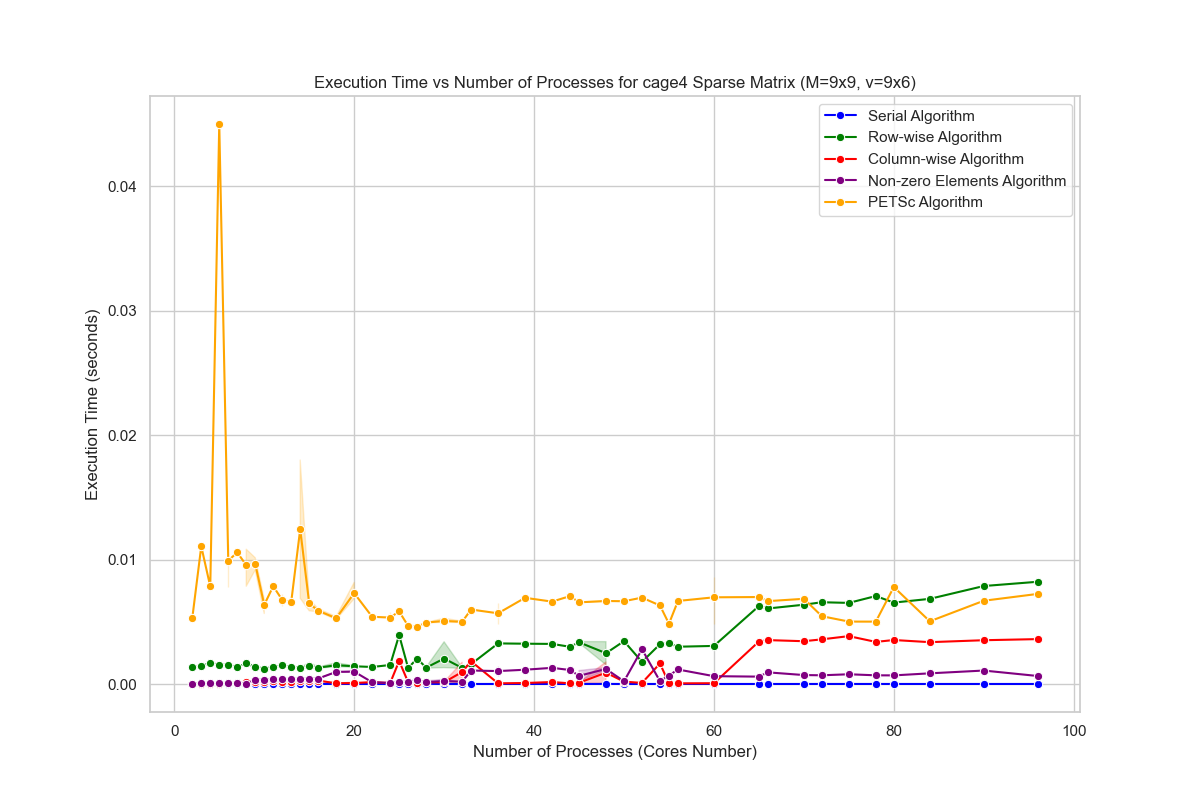
\includegraphics[width=0.5\linewidth]{../results/matrix_dim/cage4_k6_execution_time.png}
    \caption{Cage4 matrix execution time}\label{fig:cage4-k6-execution-time}
\end{figure}

\begin{figure}[H]
    \centering
    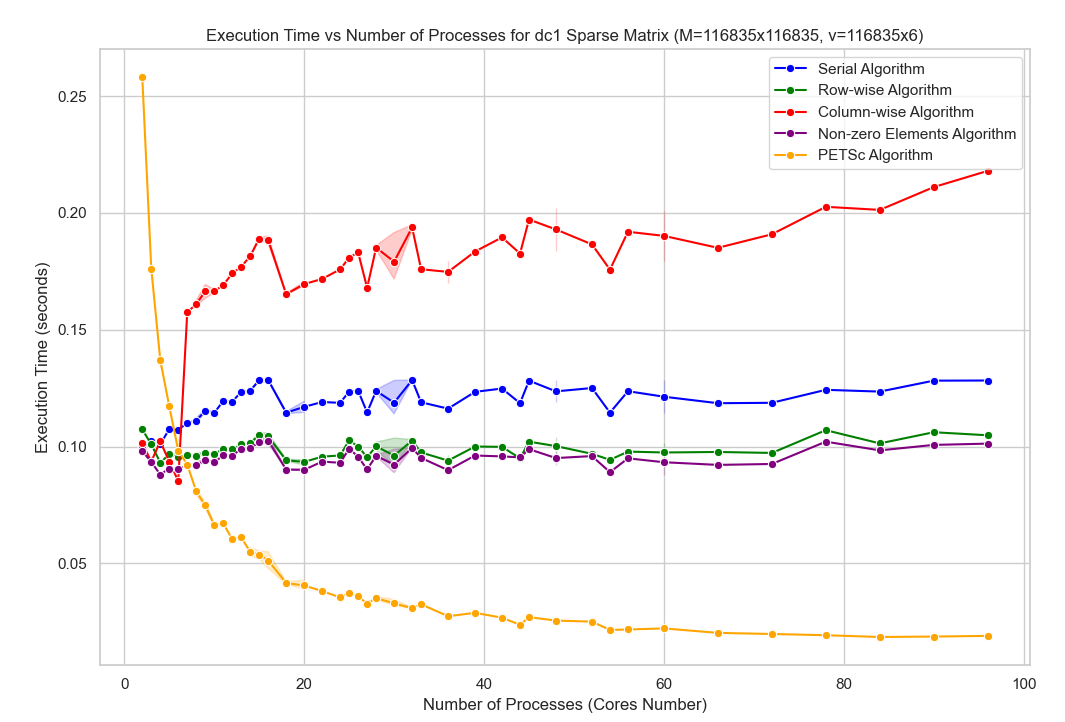
\includegraphics[width=0.6\textwidth]{../results/matrix_dim/dc1_k6_execution_time.png}
    \caption{DC1 matrix execution time}\label{fig:dc1-k6-execution-time}
\end{figure}

\begin{figure}[H]
    \centering
    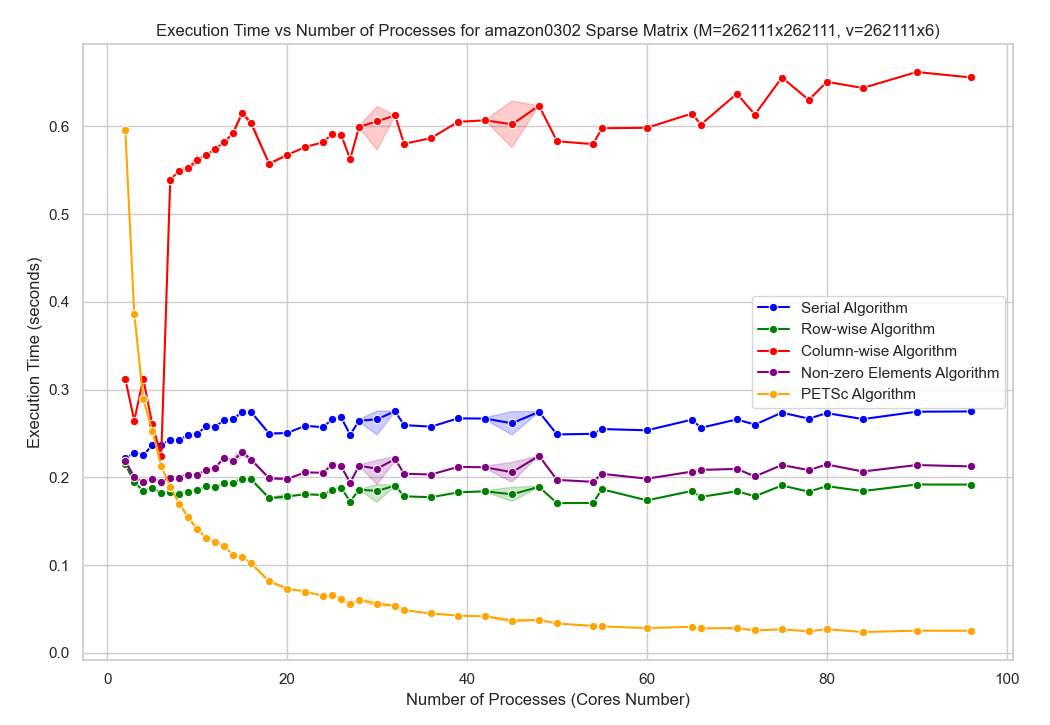
\includegraphics[width=0.6\linewidth]{../results/matrix_dim/amazon0302_k6_execution_time.png}
    \caption{Amazon0302 matrix execution time}\label{fig:amazon0302-k6-execution-time}
\end{figure}

\begin{figure}[H]
    \centering
    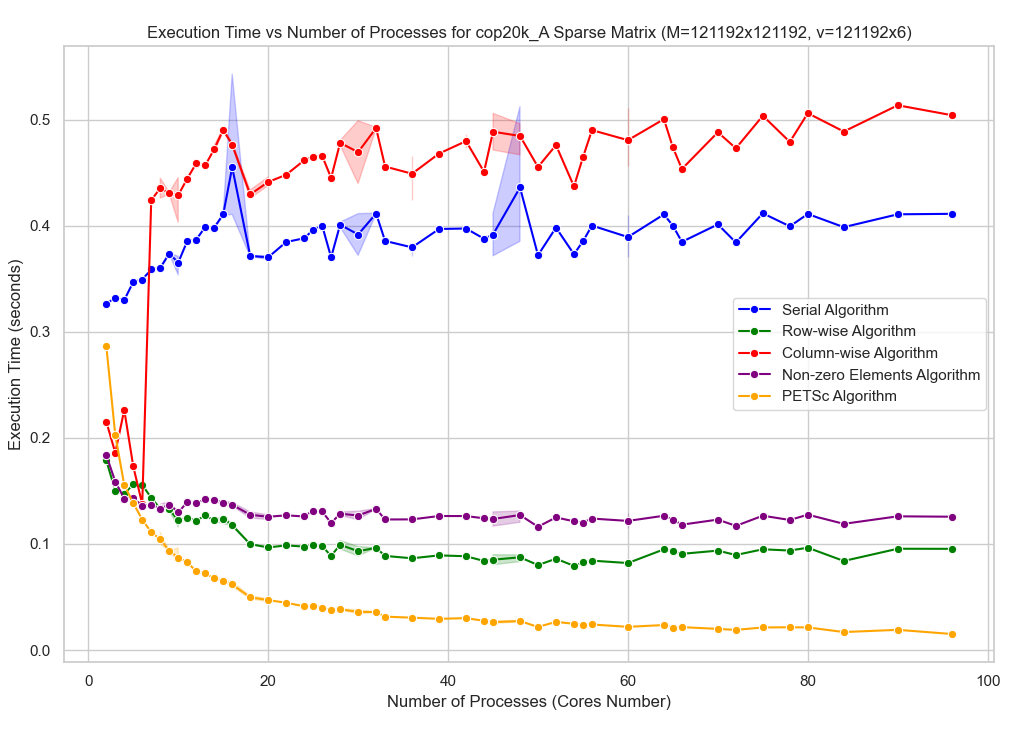
\includegraphics[width=0.6\textwidth]{../results/matrix_dim/cop20k_A_k6_execution_time.png}
    \caption{Cop20k\_A matrix execution time}\label{fig:cop20k-a-k6-execution-time}
\end{figure}

\begin{figure}[H]
    \centering
    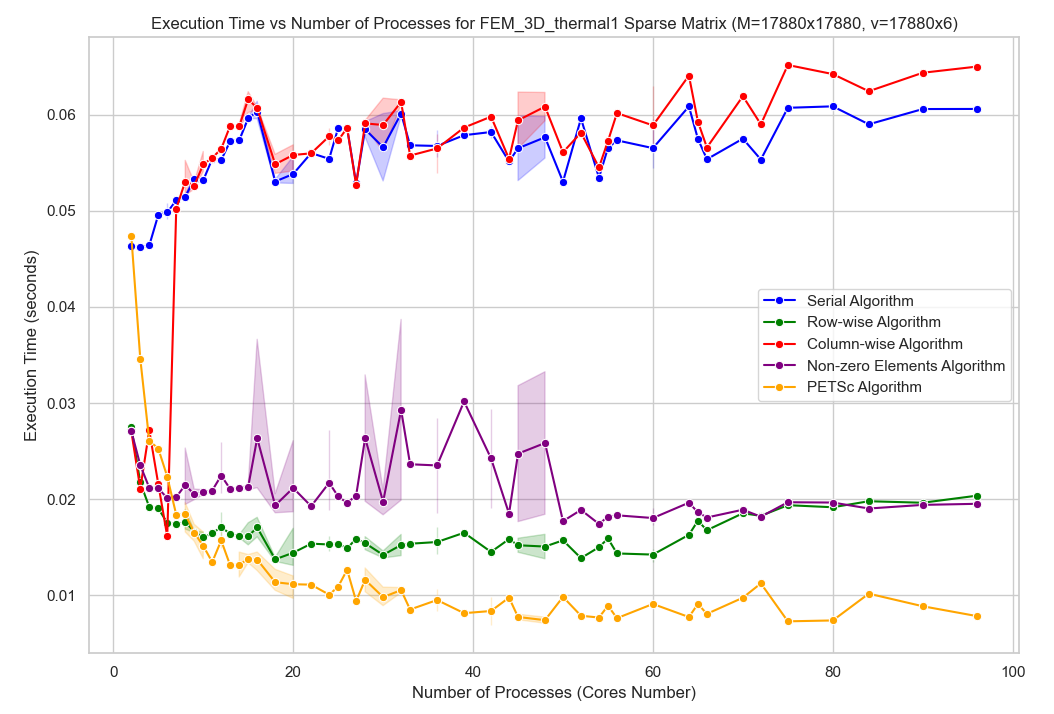
\includegraphics[width=0.6\textwidth]{../results/matrix_dim/FEM_3D_thermal1_k6_execution_time.png}
    \caption{FEM\_3D\_thermal1 matrix execution time}\label{fig:fem-3d-thermal1-k6-execution-time}
\end{figure}

\subsubsection{Communication Time}

\begin{figure}[H]
    \centering
    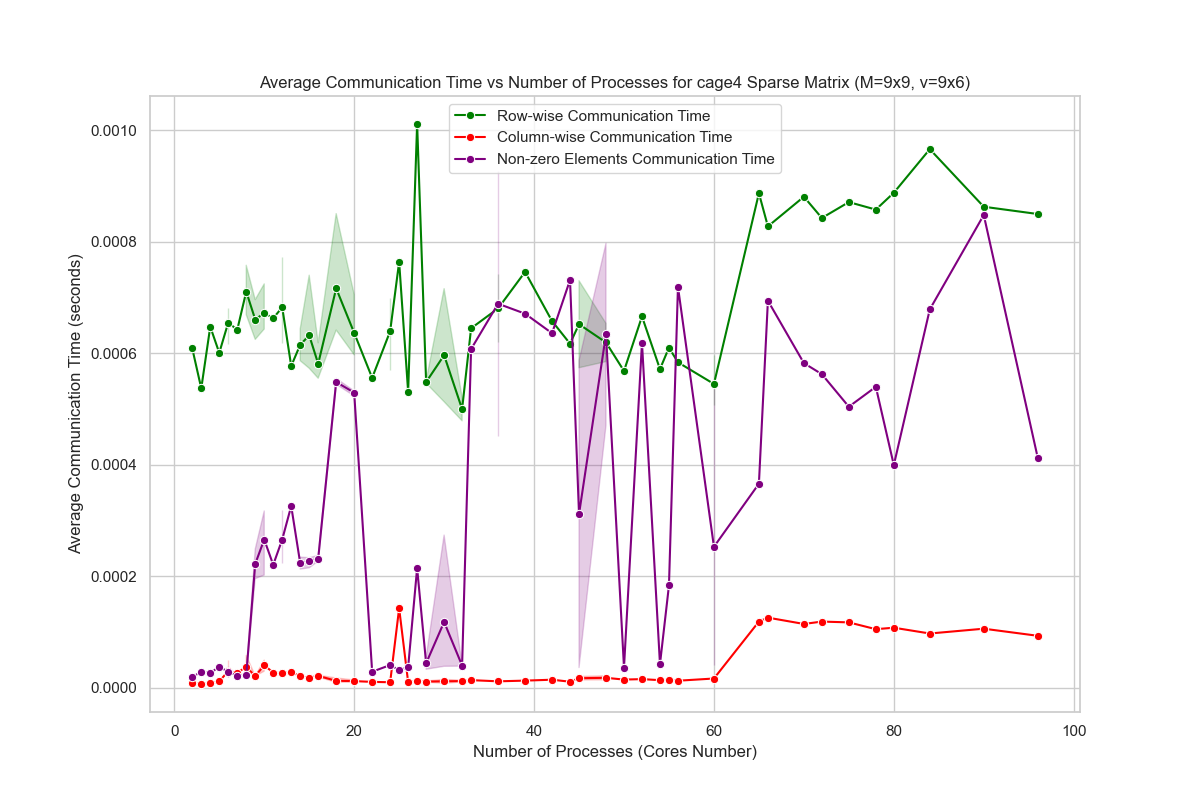
\includegraphics[width=0.5\textwidth]{../results/matrix_dim/cage4_k6_communication_time.png}
    \caption{Cage4 matrix communication time}\label{fig:cage4-k6-communication-time}
\end{figure}

\begin{figure}[H]
    \centering
    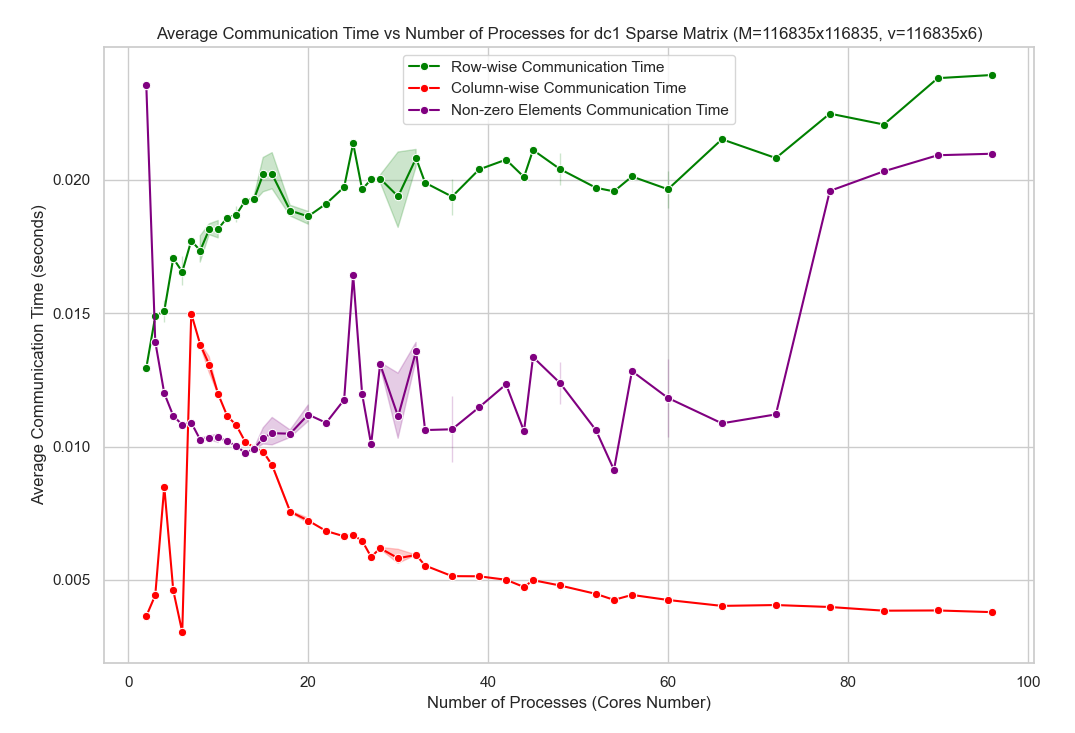
\includegraphics[width=0.5\textwidth]{../results/matrix_dim/dc1_k6_communication_time.png}
    \caption{DC1 matrix communication time}\label{fig:dc1-k6-communication-time}
\end{figure}

\begin{figure}[H]
    \centering
    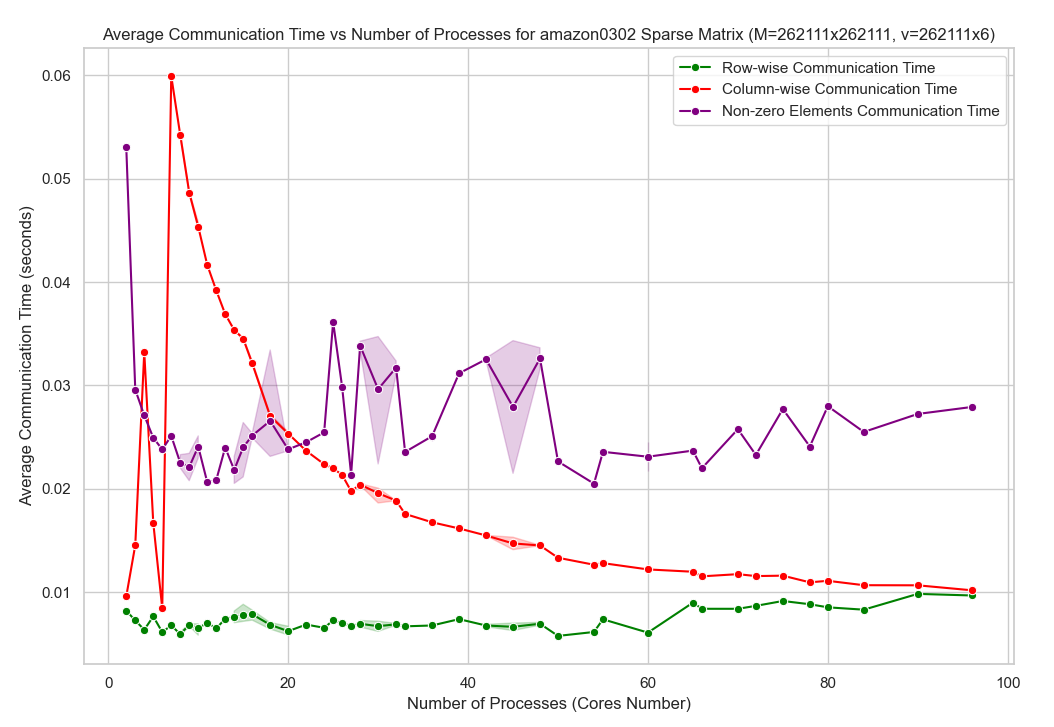
\includegraphics[width=0.5\textwidth]{../results/matrix_dim/amazon0302_k6_communication_time.png}
    \caption{Amazon0302 matrix communication time}\label{fig:amazon0302-k6-communication-time}
\end{figure}

\begin{figure}[H]
    \centering
    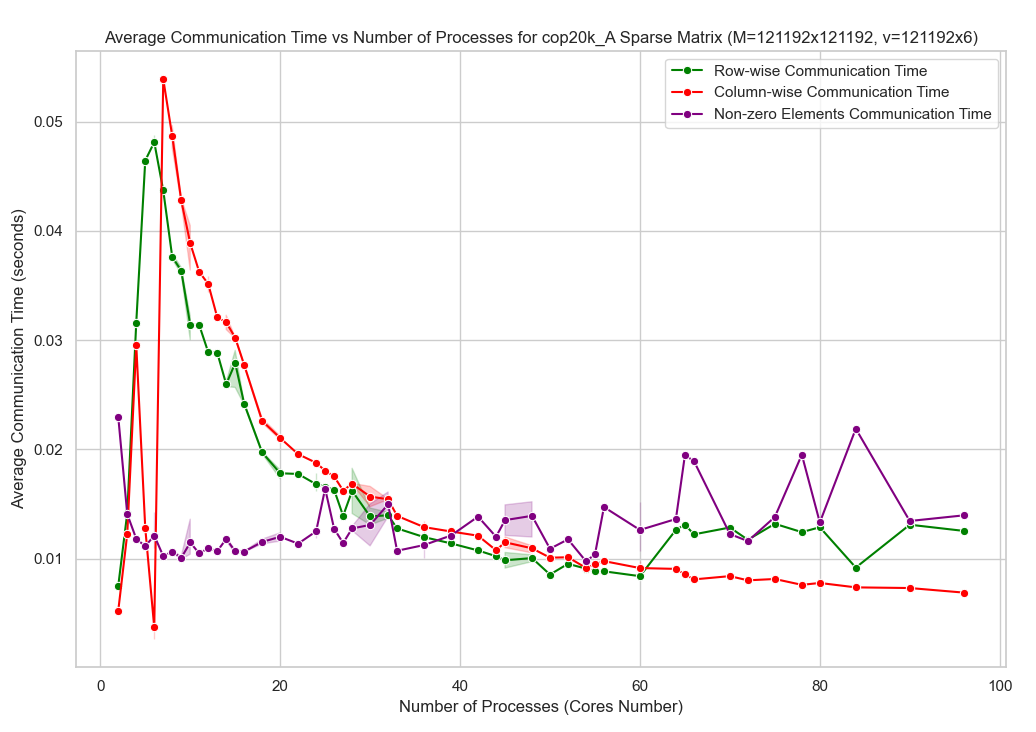
\includegraphics[width=0.5\textwidth]{../results/matrix_dim/cop20k_A_k6_communication_time.png}
    \caption{Cop20k\_A matrix communication time}\label{fig:cop20k-a-k6-communication-time-1}
\end{figure}

\begin{figure}[H]
    \centering
    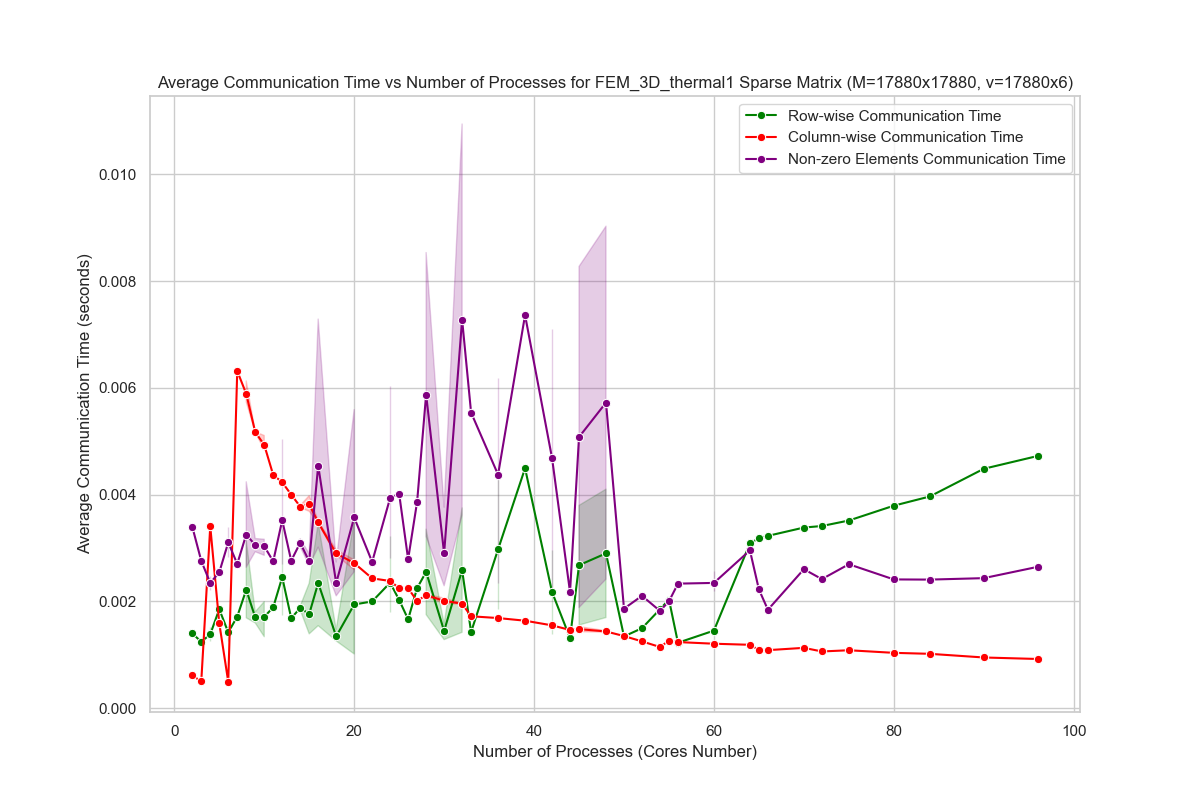
\includegraphics[width=0.5\textwidth]{../results/matrix_dim/FEM_3D_thermal1_k6_communication_time.png}
    \caption{FEM\_3D\_thermal1 matrix communication time}\label{fig:fem-3d-thermal1-k6-communication-time}
\end{figure}

\subsubsection{Computation Time}

\begin{figure}[H]
    \centering
    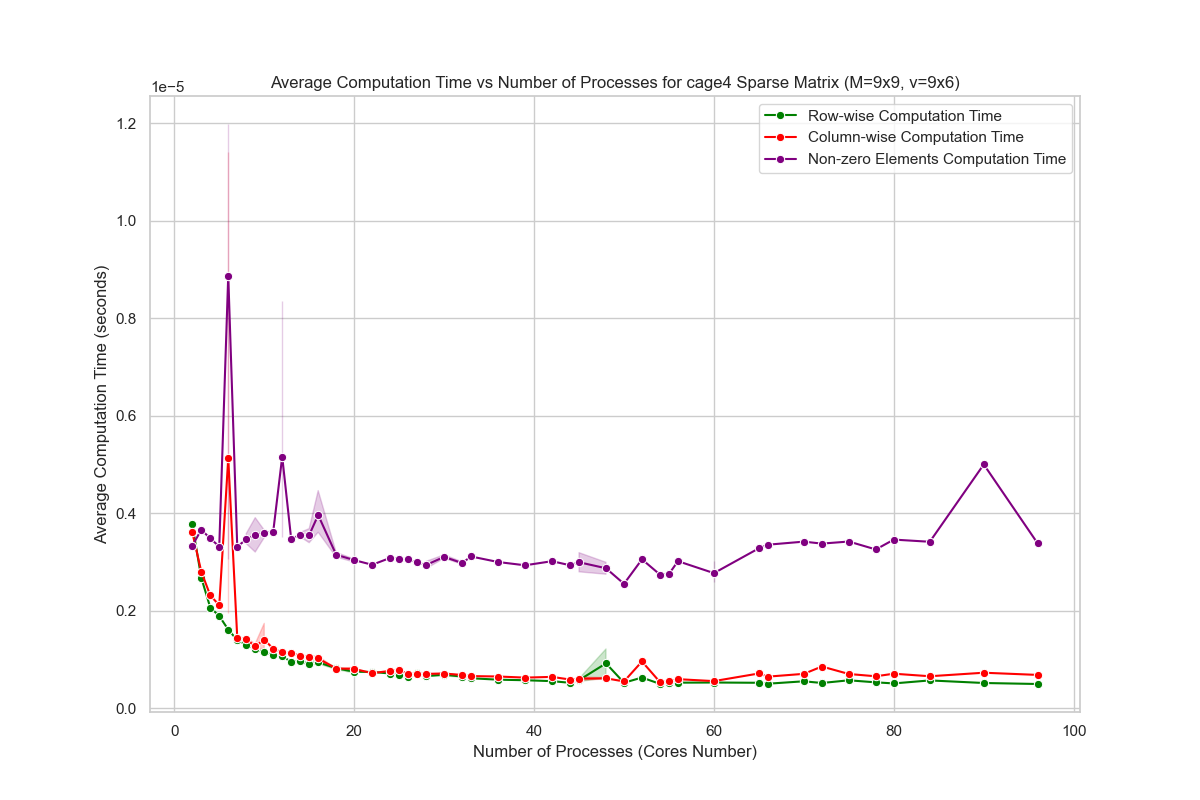
\includegraphics[width=0.5\textwidth]{../results/matrix_dim/cage4_k6_computation_time.png}
    \caption{Cage4 matrix computation time}\label{fig:cage4-k6-computation-time}
\end{figure}

\begin{figure}[H]
    \centering
    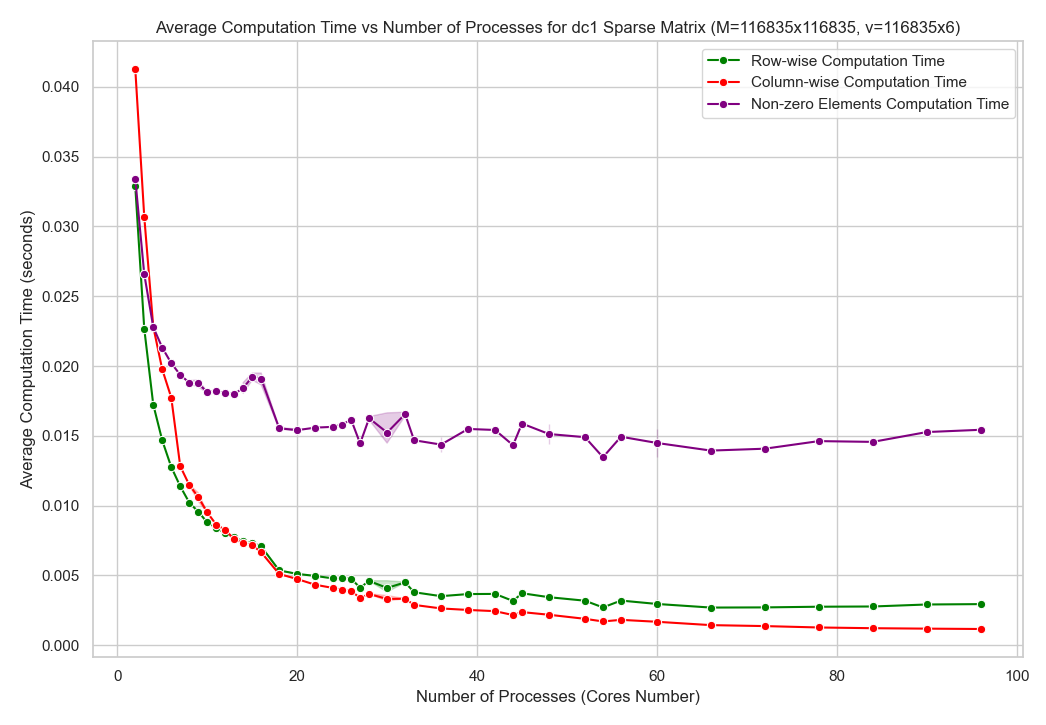
\includegraphics[width=0.5\textwidth]{../results/matrix_dim/dc1_k6_computation_time.png}
    \caption{DC1 matrix computation time}\label{fig:dc1-k6-computation-time}
\end{figure}

\begin{figure}[H]
    \centering
    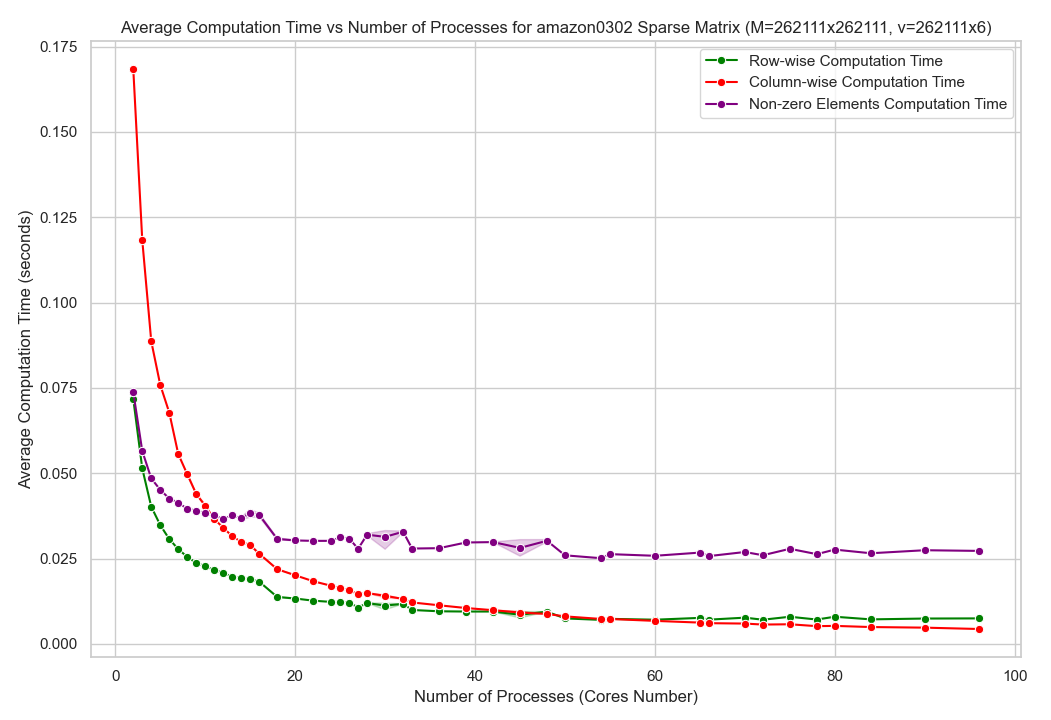
\includegraphics[width=0.5\textwidth]{../results/matrix_dim/amazon0302_k6_computation_time.png}
    \caption{Amazon0302 matrix computation time}\label{fig:amazon0302-k6-computation-time}
\end{figure}

\begin{figure}[H]
    \centering
    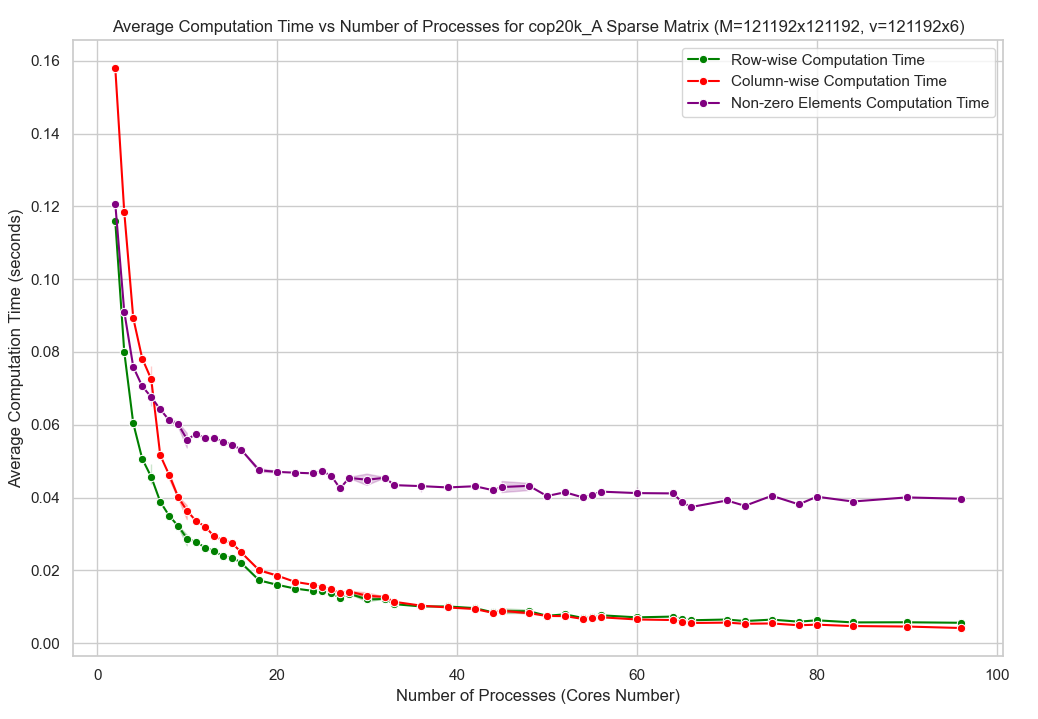
\includegraphics[width=0.5\textwidth]{../results/matrix_dim/cop20k_A_k6_computation_time.png}
    \caption{Cop20k\_A matrix computation time}\label{fig:cop20k-a-k6-computation-tim-1}
\end{figure}

\begin{figure}[H]
    \centering
    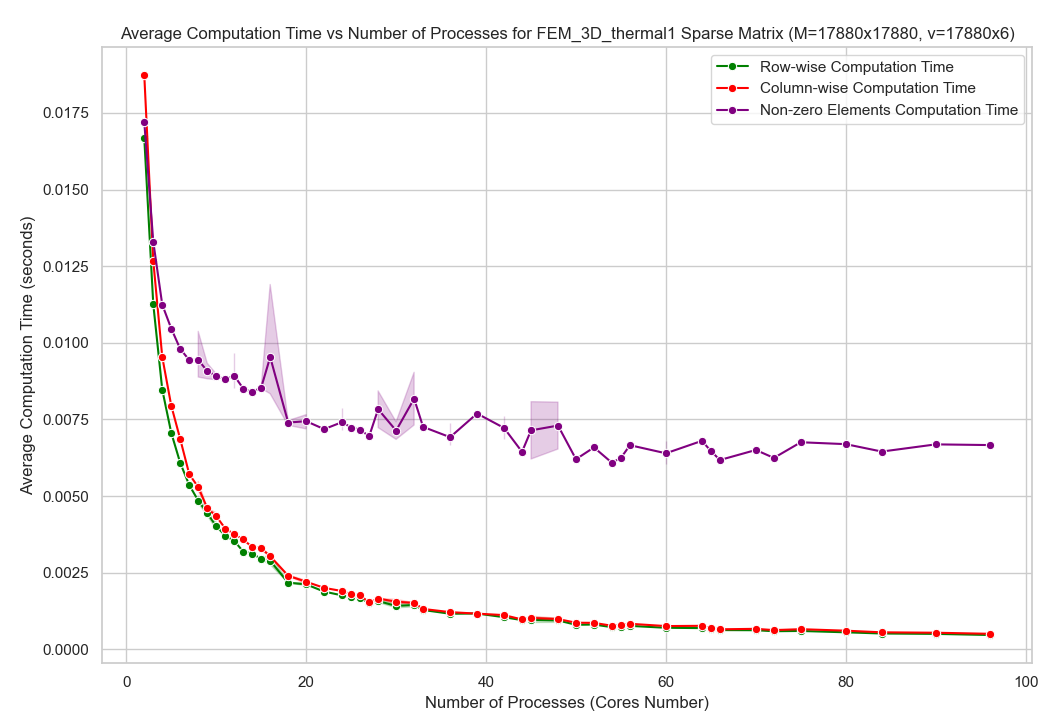
\includegraphics[width=0.5\textwidth]{../results/matrix_dim/FEM_3D_thermal1_k6_computation_time.png}
    \caption{FEM\_3D\_thermal1 matrix computation time}\label{fig:fem-3d-thermal1-k6-computation-time}
\end{figure}

\subsubsection{Performance}

\begin{figure}[H]
    \centering
    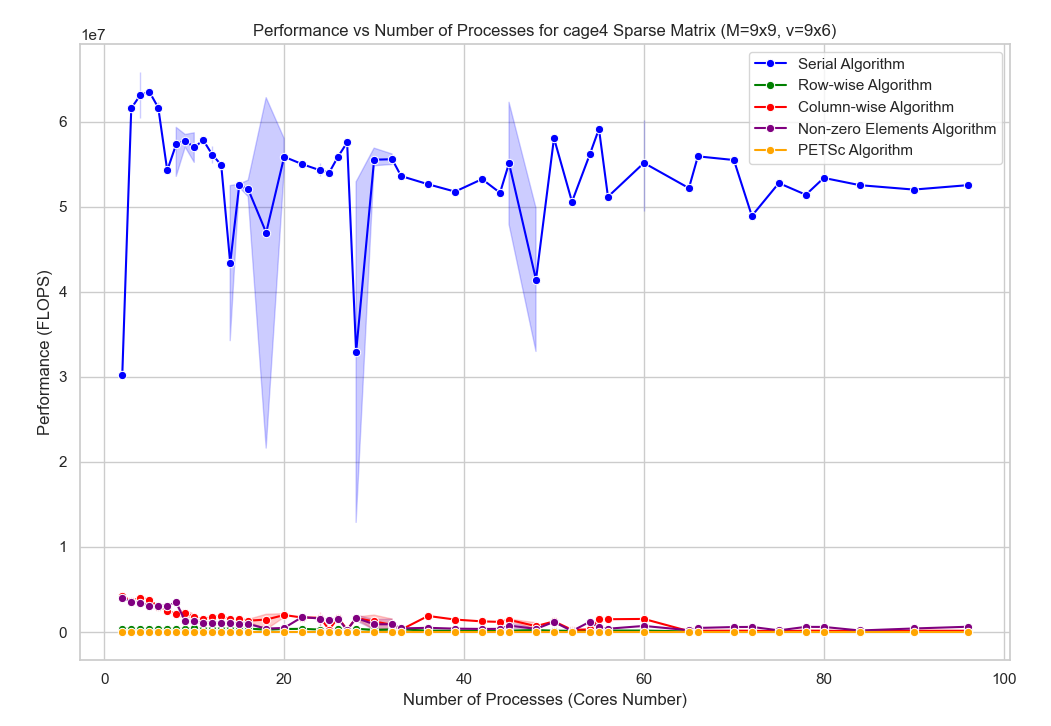
\includegraphics[width=0.5\textwidth]{../results/matrix_dim/cage4_k6_performance.png}
    \caption{Cage4 matrix performance}\label{fig:cage4-k6-performance}
\end{figure}

\begin{figure}[H]
    \centering
    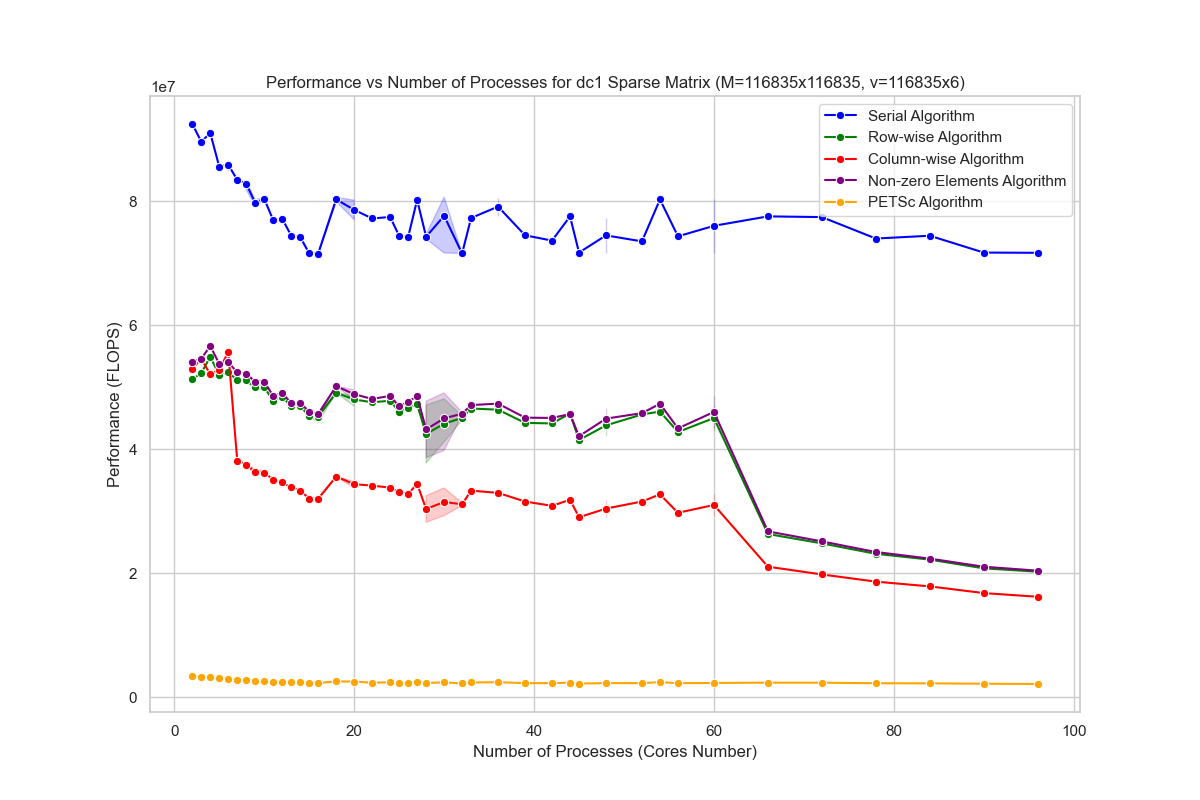
\includegraphics[width=0.5\textwidth]{../results/matrix_dim/dc1_k6_performance.png}
    \caption{DC1 matrix performance}\label{fig:dc1-k6-performance}
\end{figure}

\begin{figure}[H]
    \centering
    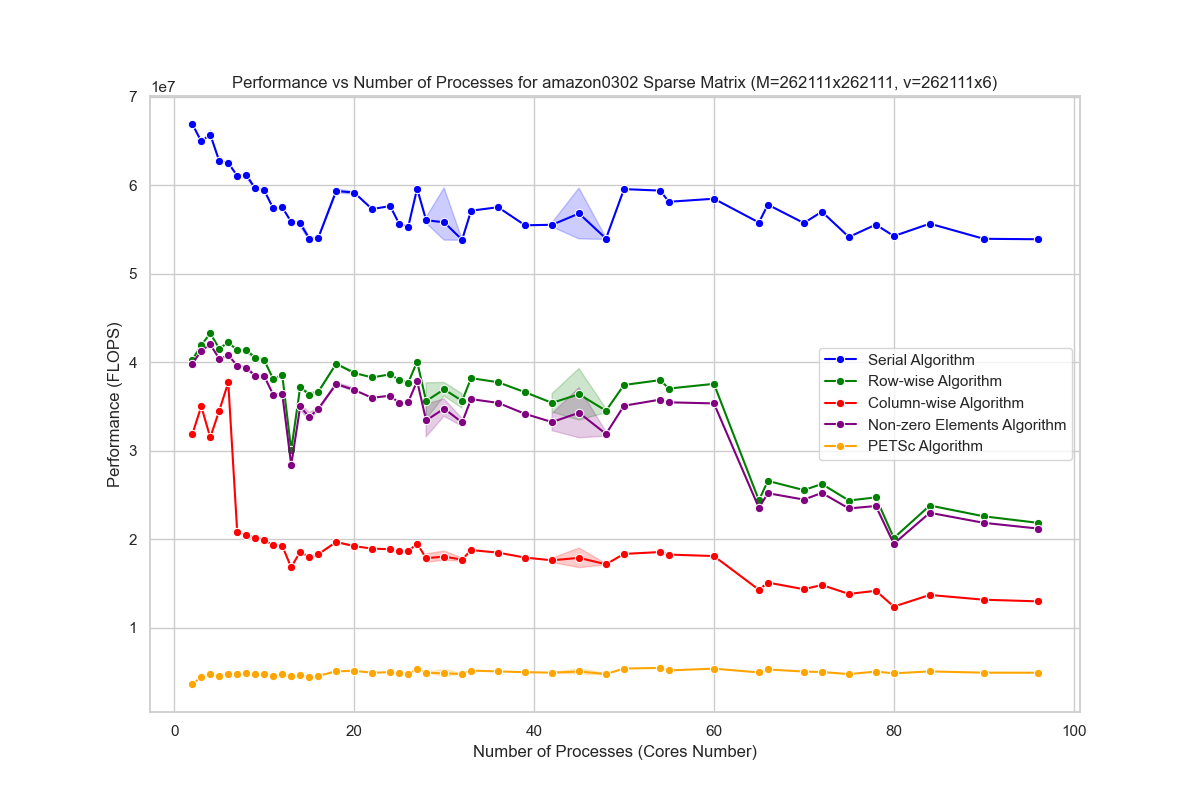
\includegraphics[width=0.5\textwidth]{../results/matrix_dim/amazon0302_k6_performance.png}
    \caption{Amazon0302 matrix performance}\label{fig:amazon0302-k6-performance}
\end{figure}

\begin{figure}[H]
    \centering
    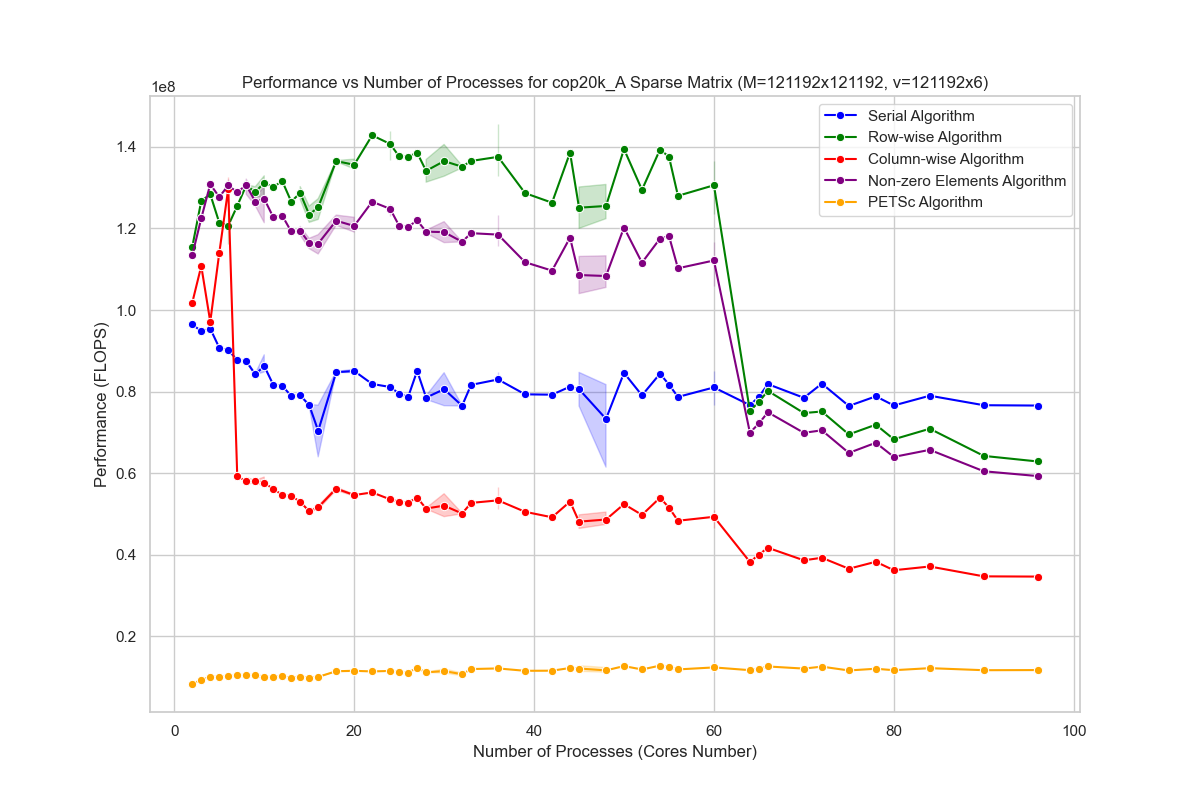
\includegraphics[width=0.5\textwidth]{../results/matrix_dim/cop20k_A_k6_performance.png}
    \caption{Cop20k\_A matrix performance}\label{fig:cop20k-a-k6-performance-1}
\end{figure}

\begin{figure}[H]
    \centering
    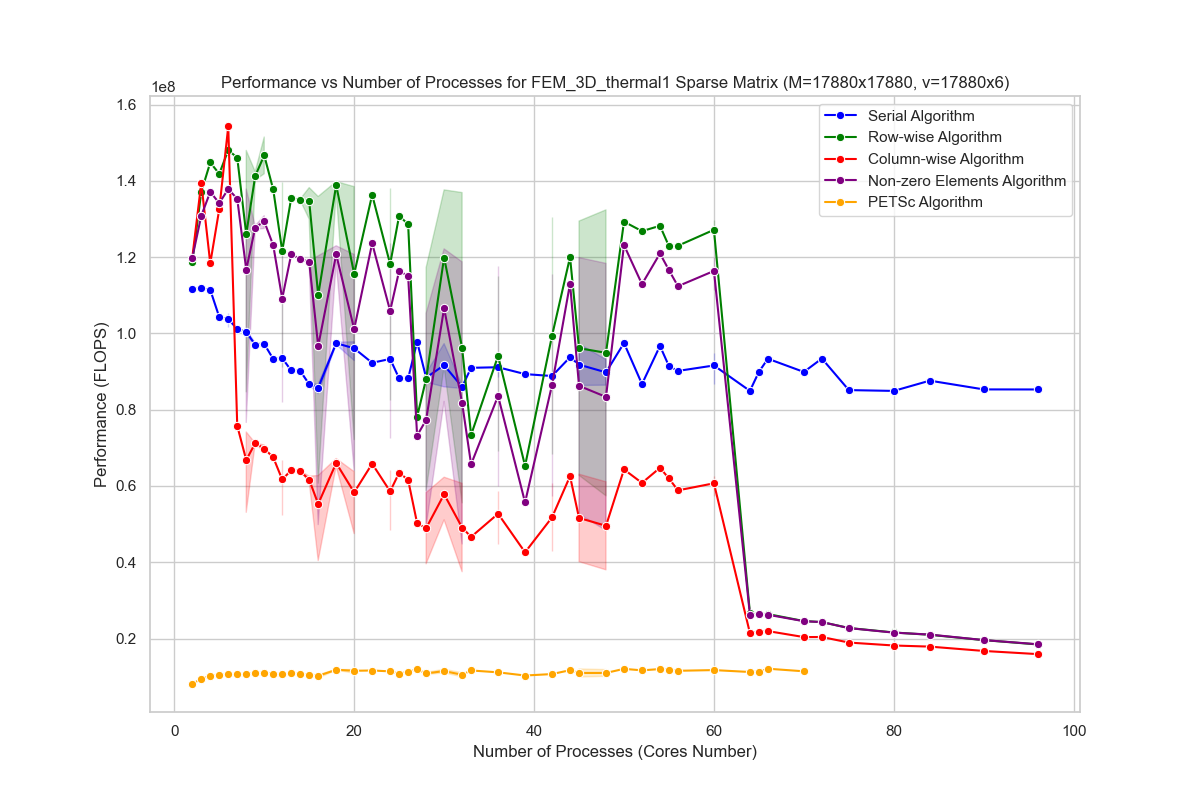
\includegraphics[width=0.5\textwidth]{../results/matrix_dim/FEM_3D_thermal1_k6_performance.png}
    \caption{FEM\_3D\_thermal1 matrix performance}\label{fig:fem-3d-thermal1-k6-performance}
\end{figure}

\subsection{Fat Vector Impact}
\subsubsection{Execution Time}

\begin{figure}[H]
    \centering
    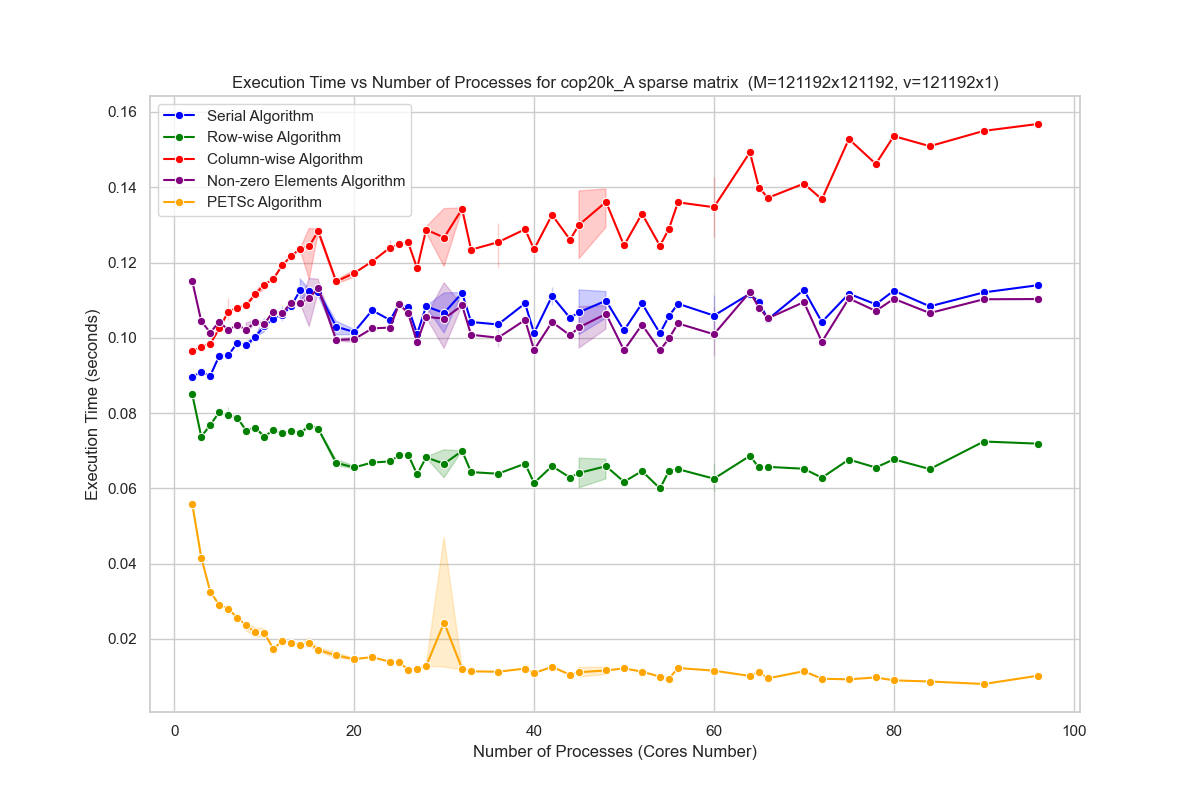
\includegraphics[width=0.5\textwidth]{../results/fat_vector_dim/cop20k_A_k1_execution_time.png}
    \caption{Cop20k\_A matrix execution time}\label{fig:cop20k-a-k1-execution-time}
\end{figure}

\begin{figure}[H]
    \centering
    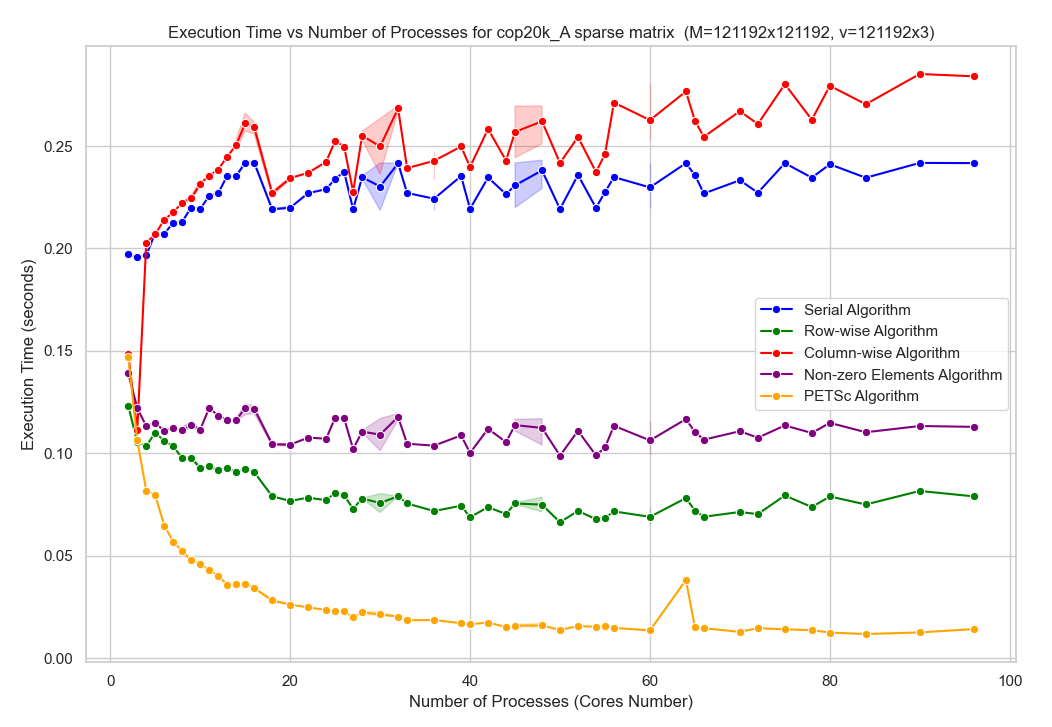
\includegraphics[width=0.5\textwidth]{../results/fat_vector_dim/cop20k_A_k3_execution_time.png}
    \caption{Cop20k\_A matrix execution time}\label{fig:cop20k-a-k3-execution-time}
\end{figure}

\begin{figure}[H]
    \centering
    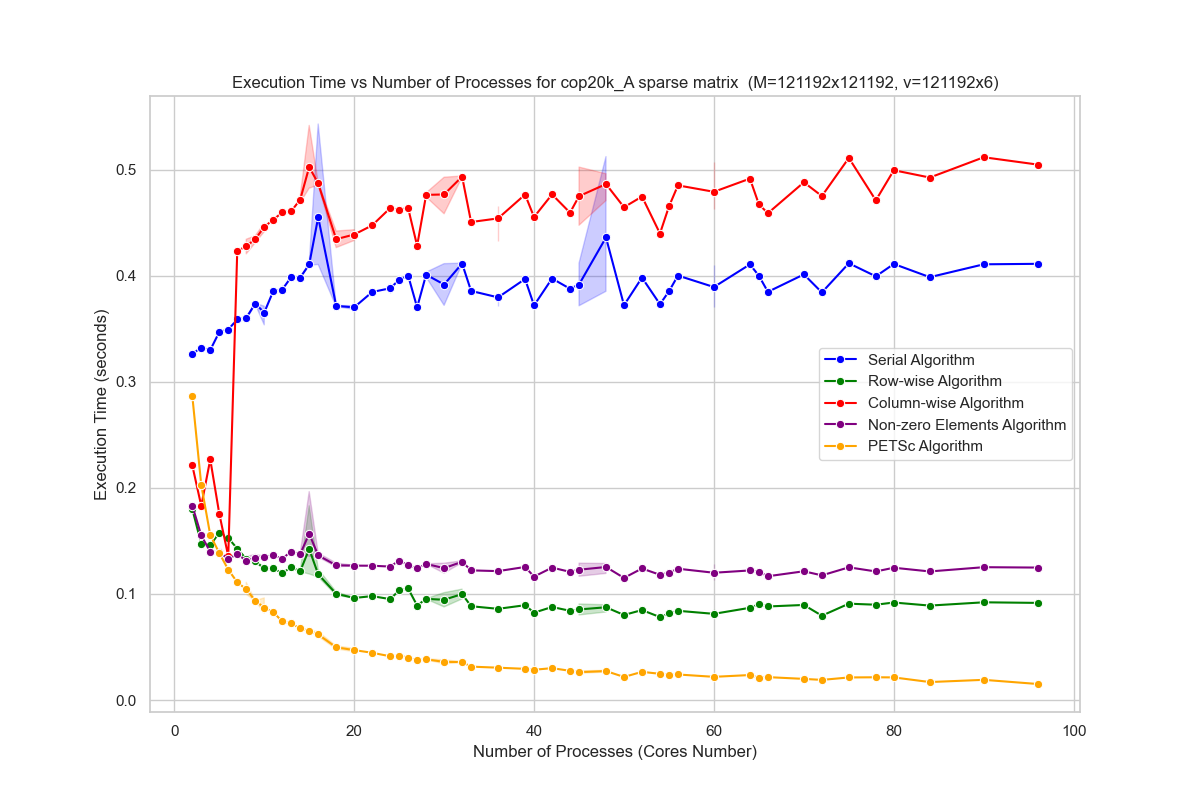
\includegraphics[width=0.5\textwidth]{../results/fat_vector_dim/cop20k_A_k6_execution_time.png}
    \caption{Cop20k\_A matrix execution time}\label{fig:cop20k-a-k6-execution-time-2}
\end{figure}

\begin{figure}[H]
    \centering
    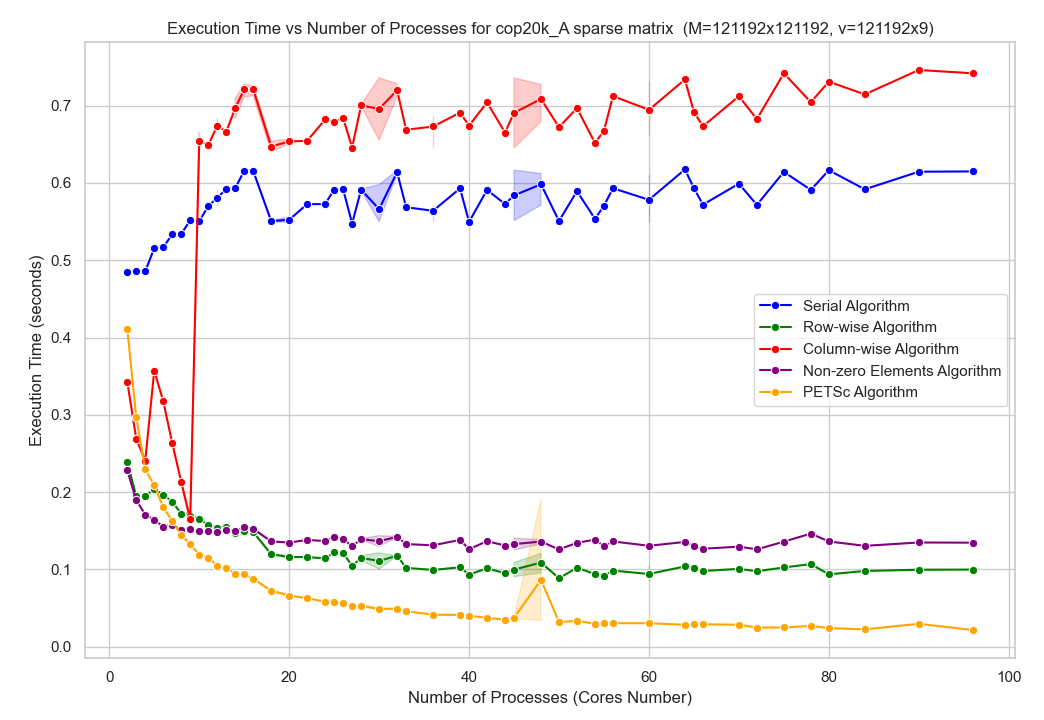
\includegraphics[width=0.5\textwidth]{../results/fat_vector_dim/cop20k_A_k9_execution_time.png}
    \caption{Cop20k\_A matrix execution time}\label{fig:cop20k-a-k9-execution-time}
\end{figure}

\begin{figure}[H]
    \centering
    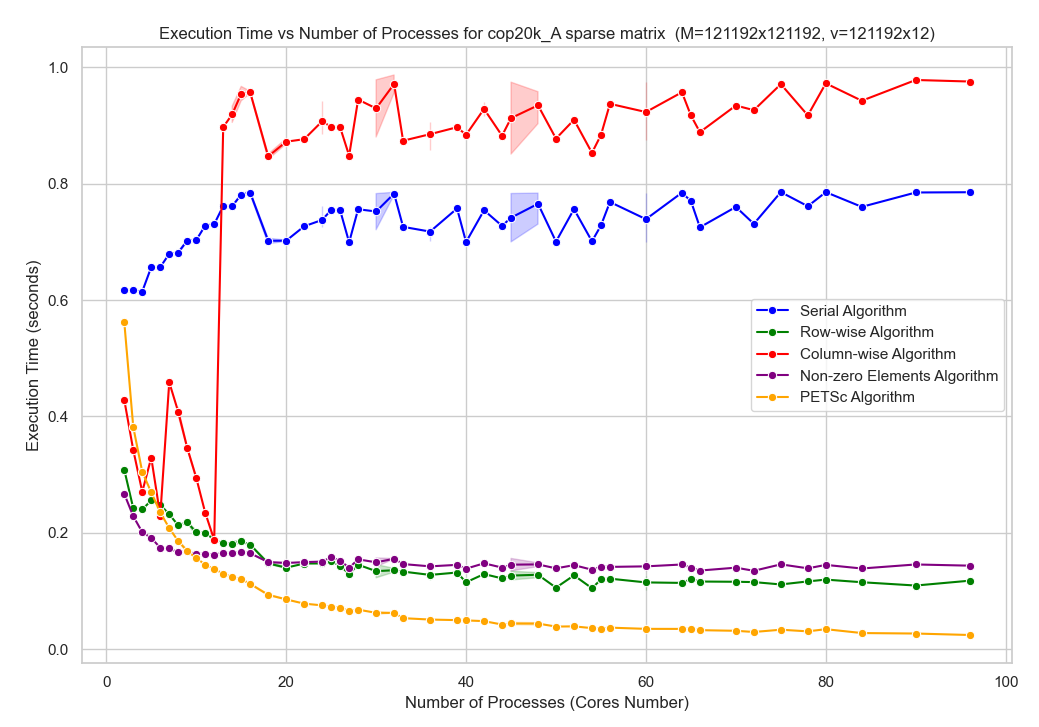
\includegraphics[width=0.5\textwidth]{../results/fat_vector_dim/cop20k_A_k12_execution_time.png}
    \caption{Cop20k\_A matrix execution time}\label{fig:cop20k-a-k12-execution-time}
\end{figure}

\subsubsection{Communication Time}

\begin{figure}[H]
    \centering
    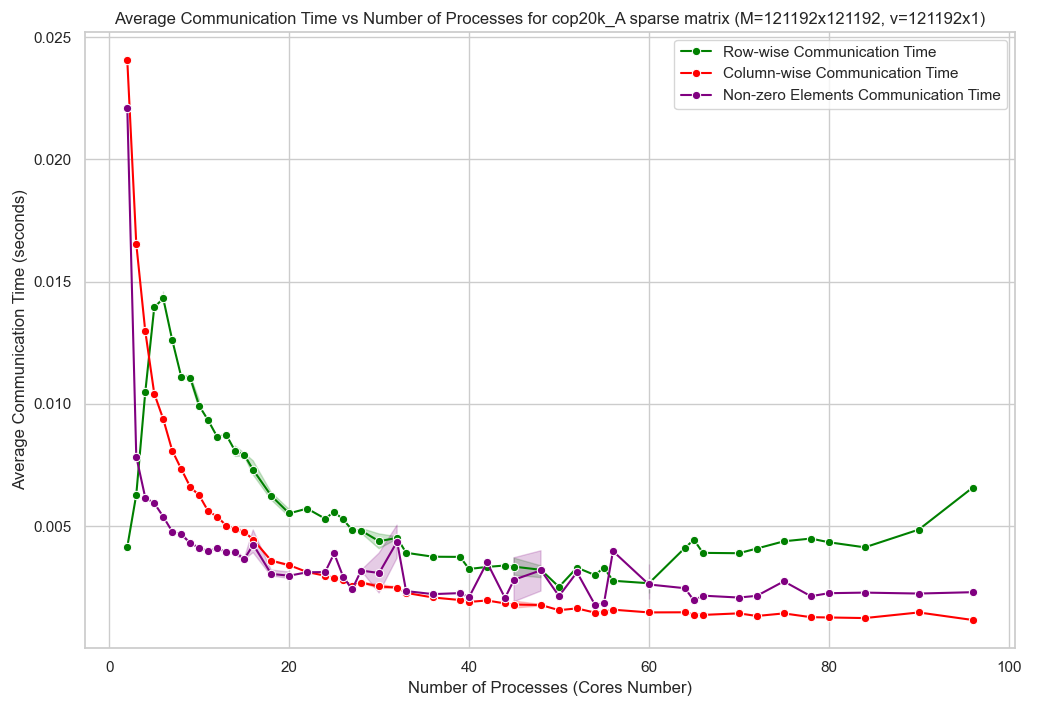
\includegraphics[width=0.5\textwidth]{../results/fat_vector_dim/cop20k_A_k1_communication_time.png}
    \caption{Cop20k\_A matrix communication time}\label{fig:cop20k-a-k1-communication-time}
\end{figure}

\begin{figure}[H]
    \centering
    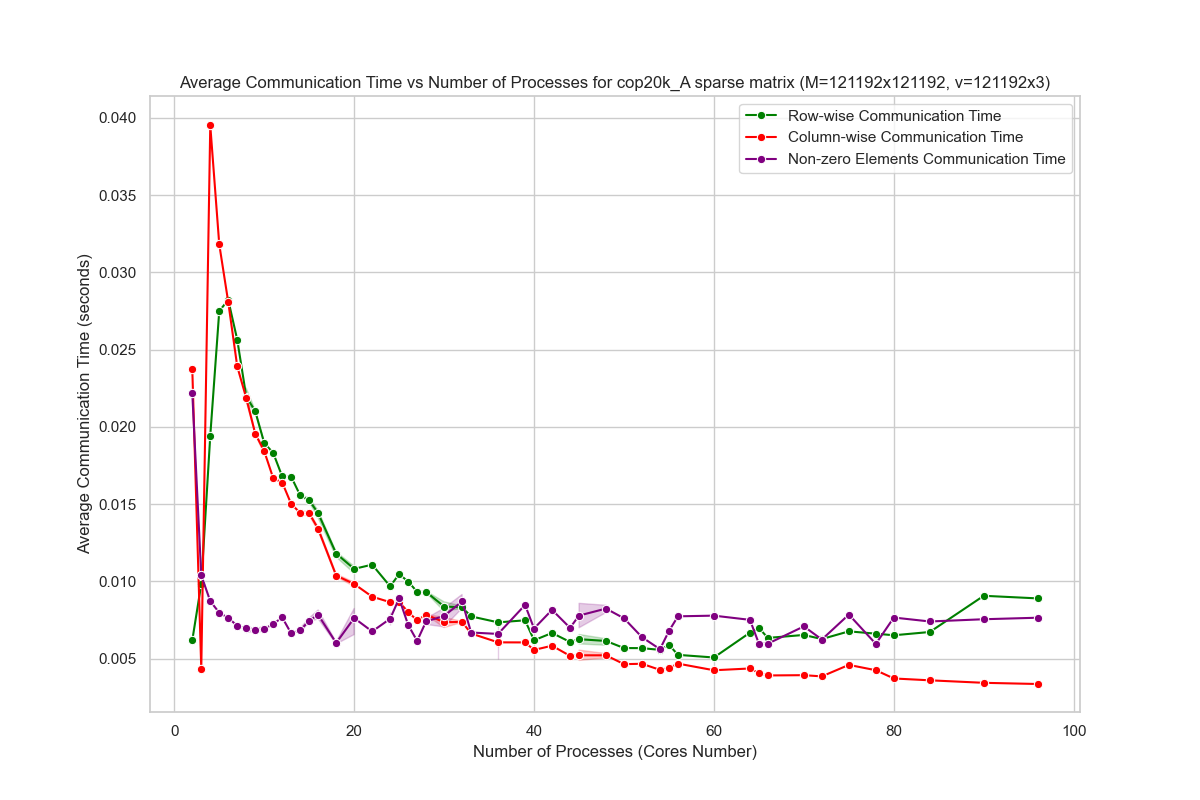
\includegraphics[width=0.5\textwidth]{../results/fat_vector_dim/cop20k_A_k3_communication_time.png}
    \caption{Cop20k\_A matrix communication time}\label{fig:cop20k-a-k3-communication-time}
\end{figure}

\begin{figure}[H]
    \centering
    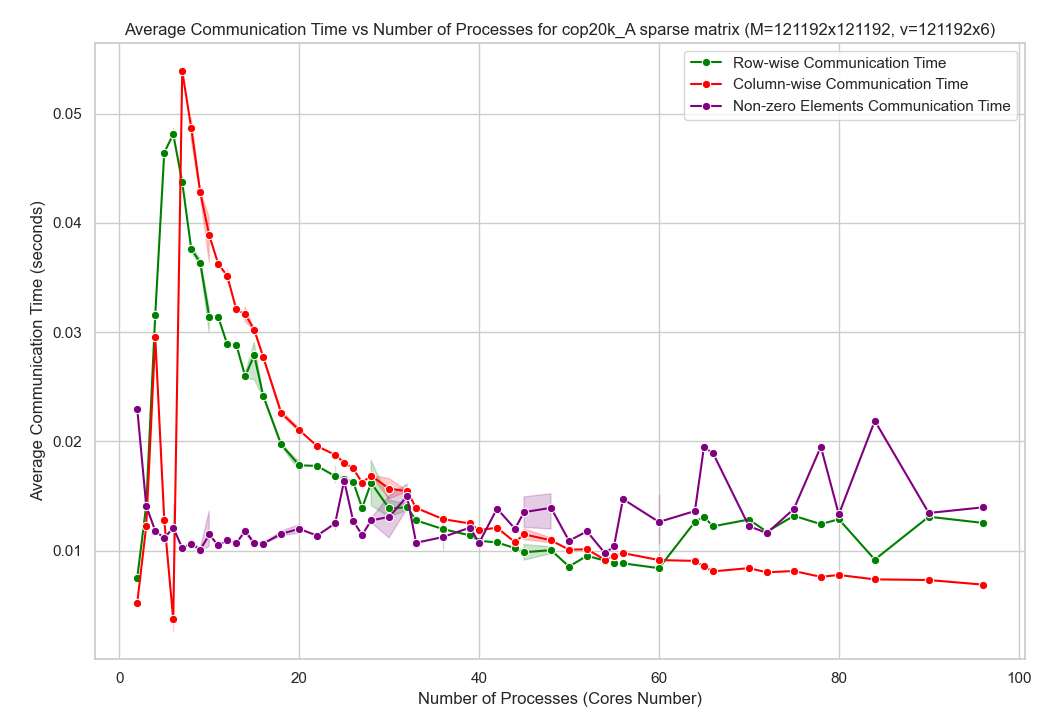
\includegraphics[width=0.5\textwidth]{../results/fat_vector_dim/cop20k_A_k6_communication_time.png}
    \caption{Cop20k\_A matrix communication time}\label{fig:cop20k-a-k6-communication-time}
\end{figure}

\begin{figure}[H]
    \centering
    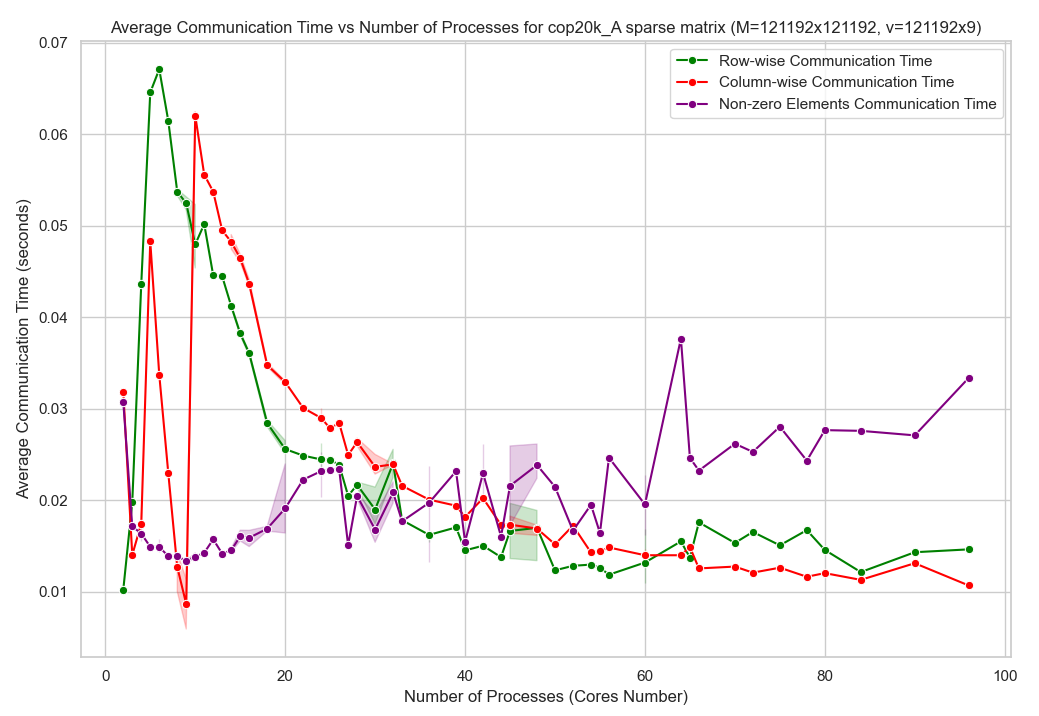
\includegraphics[width=0.5\textwidth]{../results/fat_vector_dim/cop20k_A_k9_communication_time.png}
    \caption{Cop20k\_A matrix communication time}\label{fig:cop20k-a-k9-communication-time}
\end{figure}

\begin{figure}[H]
    \centering
    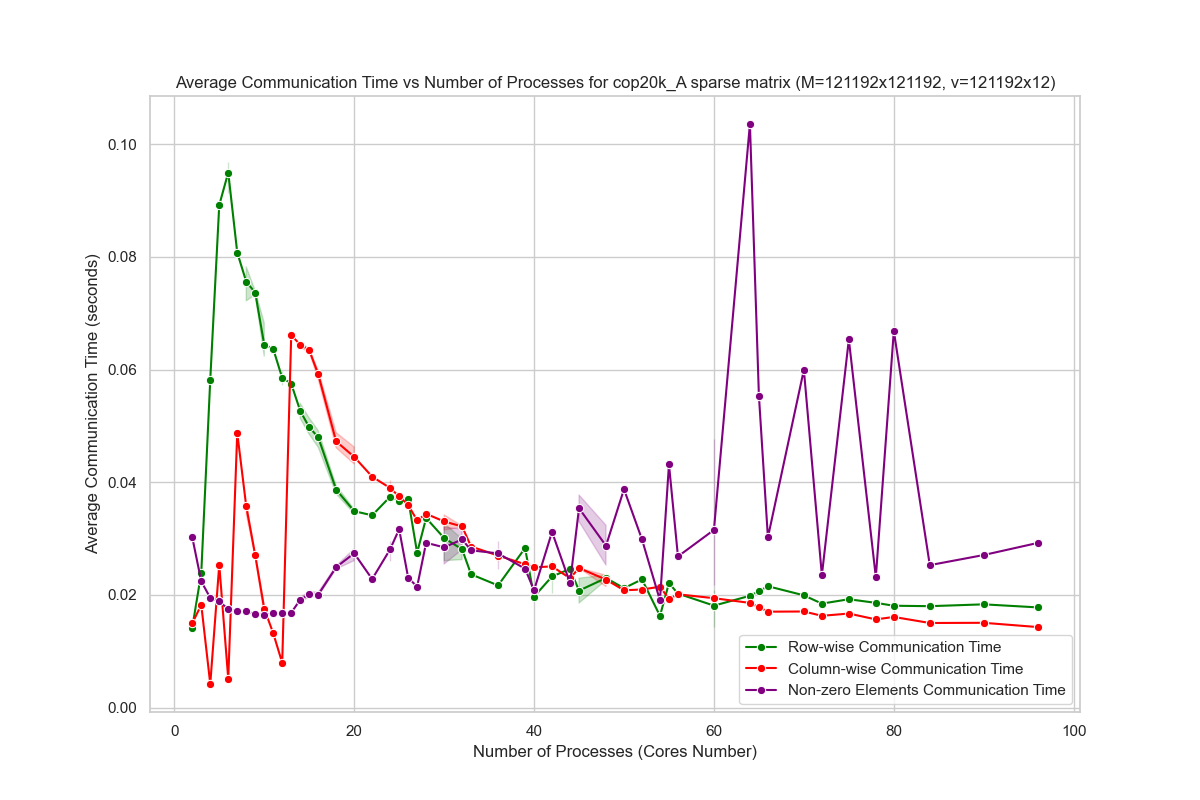
\includegraphics[width=0.5\textwidth]{../results/fat_vector_dim/cop20k_A_k12_communication_time.png}
    \caption{Cop20k\_A matrix communication time}\label{fig:cop20k-a-k12-communication-time}
\end{figure}

\subsubsection{Computation Time}

\begin{figure}[H]
    \centering
    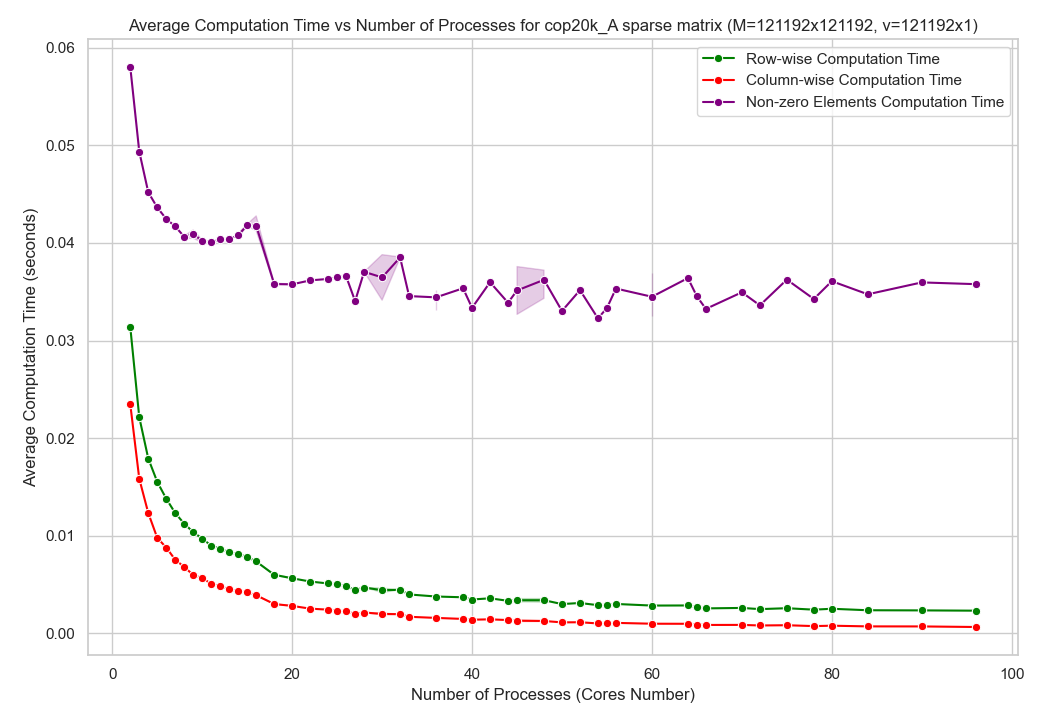
\includegraphics[width=0.5\textwidth]{../results/fat_vector_dim/cop20k_A_k1_computation_time.png}
    \caption{Cop20k\_A matrix computation time}\label{fig:cop20k-a-k1-computation-time}
\end{figure}

\begin{figure}[H]
    \centering
    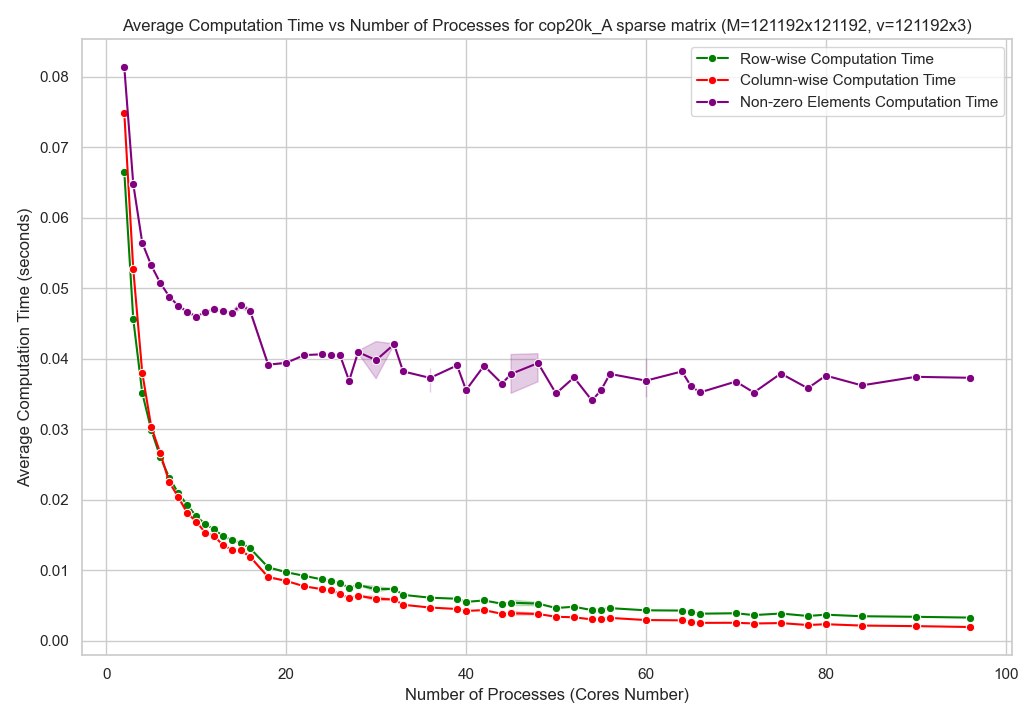
\includegraphics[width=0.5\textwidth]{../results/fat_vector_dim/cop20k_A_k3_computation_time.png}
    \caption{Cop20k\_A matrix computation time}\label{fig:cop20k-a-k3-computation-time}
\end{figure}

\begin{figure}[H]
    \centering
    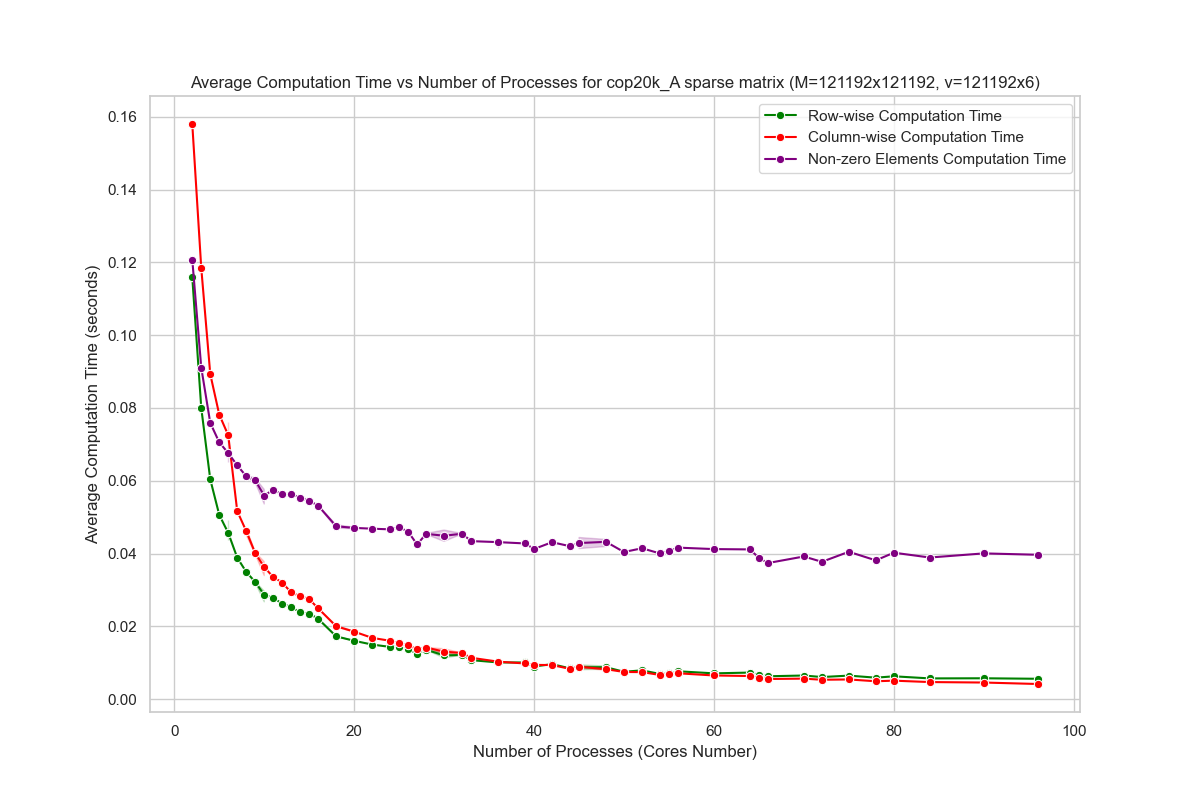
\includegraphics[width=0.5\textwidth]{../results/fat_vector_dim/cop20k_A_k6_computation_time.png}
    \caption{Cop20k\_A matrix computation time}\label{fig:cop20k-a-k6-computation-time}
\end{figure}

\begin{figure}[H]
    \centering
    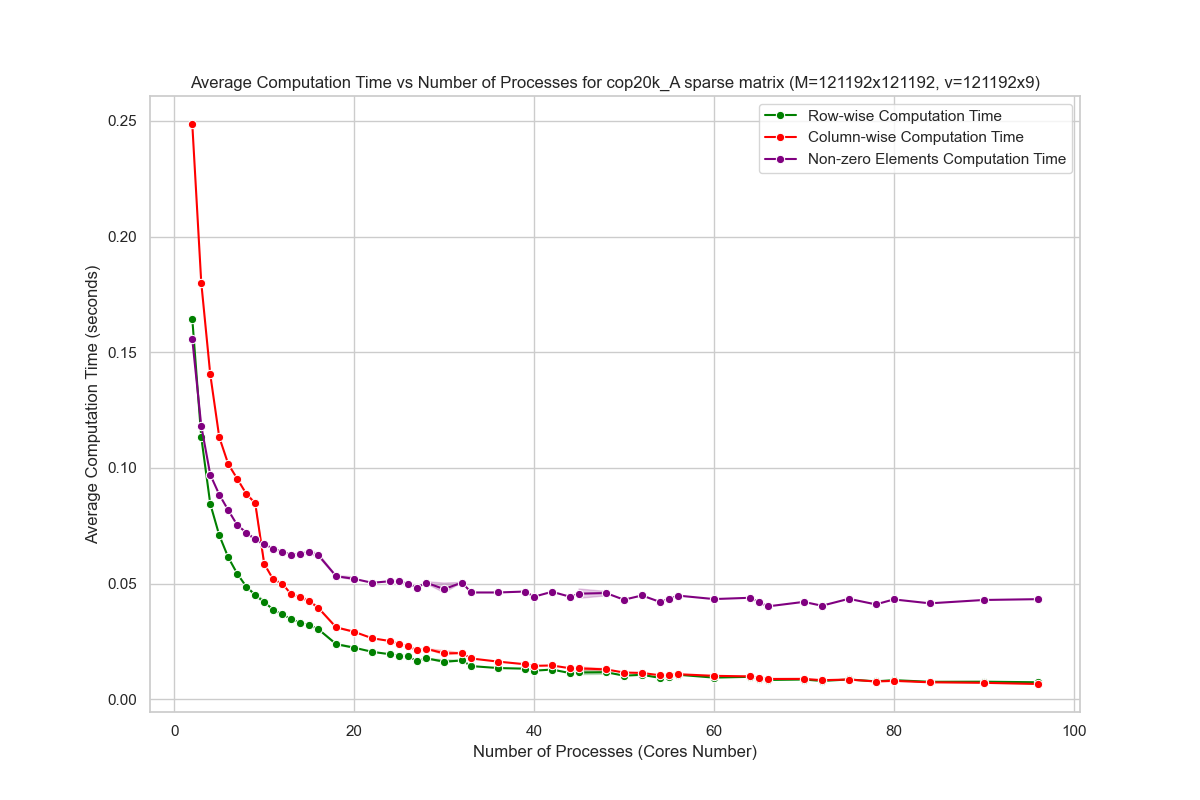
\includegraphics[width=0.5\textwidth]{../results/fat_vector_dim/cop20k_A_k9_computation_time.png}
    \caption{Cop20k\_A matrix computation time}\label{fig:cop20k-a-k9-computation-time}
\end{figure}

\begin{figure}[H]
    \centering
    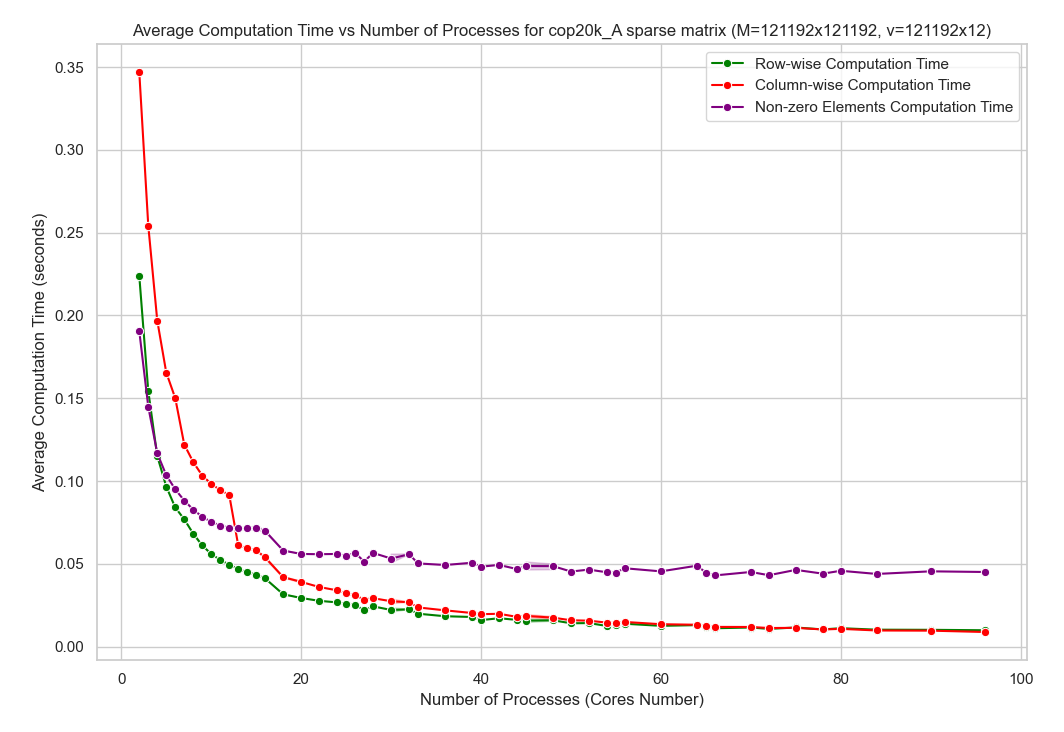
\includegraphics[width=0.5\textwidth]{../results/fat_vector_dim/cop20k_A_k12_computation_time.png}
    \caption{Cop20k\_A matrix computation time}\label{fig:cop20k-a-k12-computation-time}
\end{figure}

\subsubsection{Performance}

\begin{figure}[H]
    \centering
    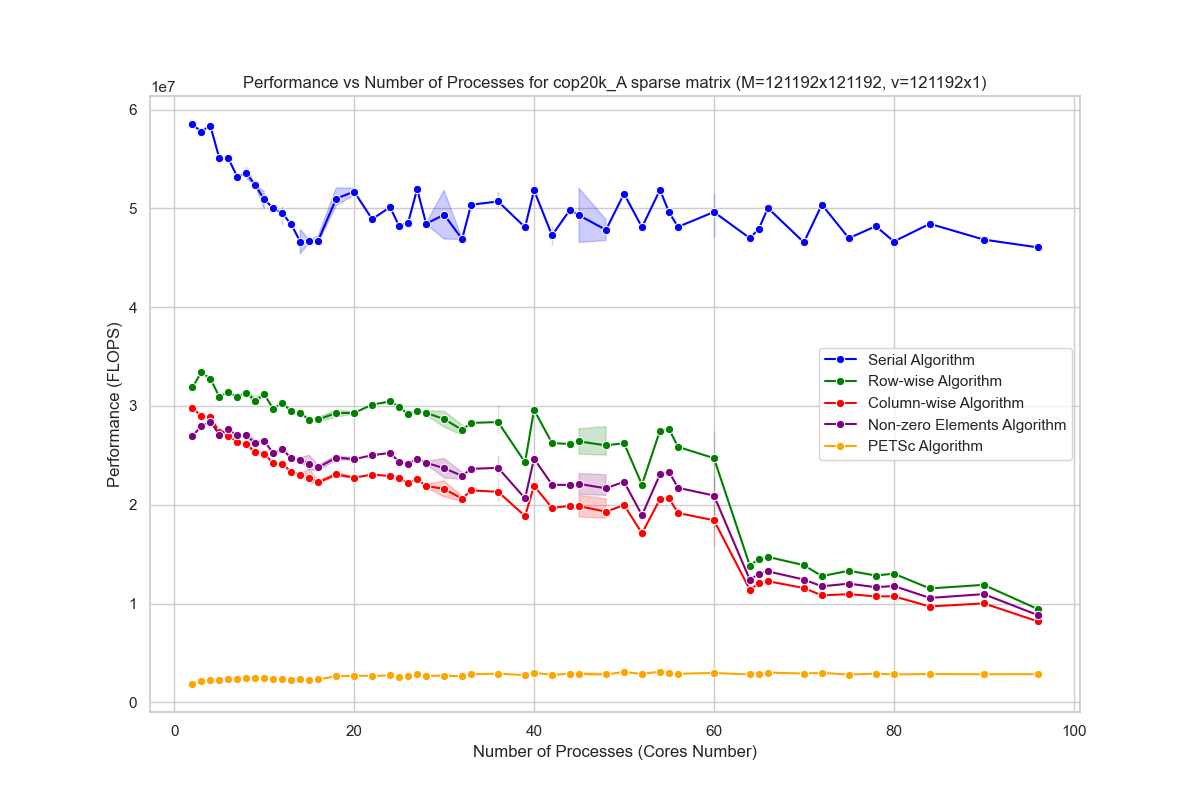
\includegraphics[width=0.5\textwidth]{../results/fat_vector_dim/cop20k_A_k1_performance.png}
    \caption{Cop20k\_A matrix performance}\label{fig:cop20k-a-k1-performance}
\end{figure}

\begin{figure}[H]
    \centering
    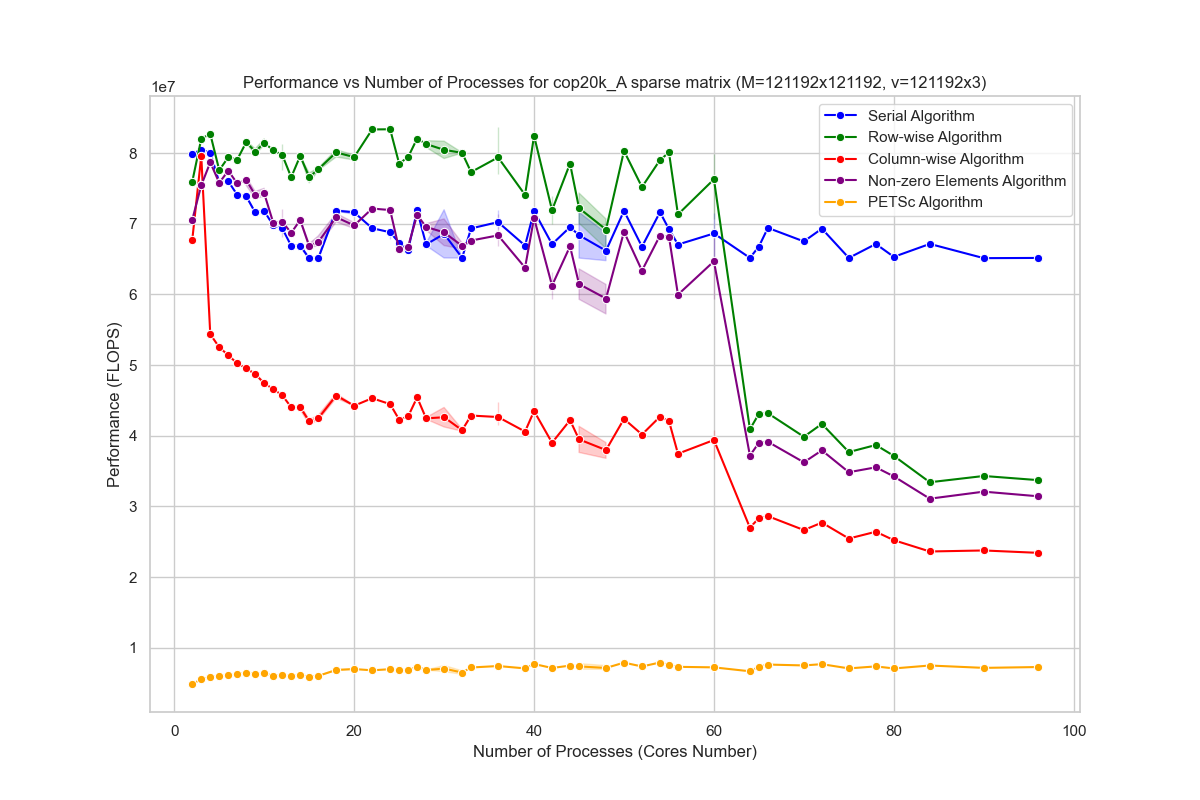
\includegraphics[width=0.5\textwidth]{../results/fat_vector_dim/cop20k_A_k3_performance.png}
    \caption{Cop20k\_A matrix performance}\label{fig:cop20k-a-k3-performance}
\end{figure}

\begin{figure}[H]
    \centering
    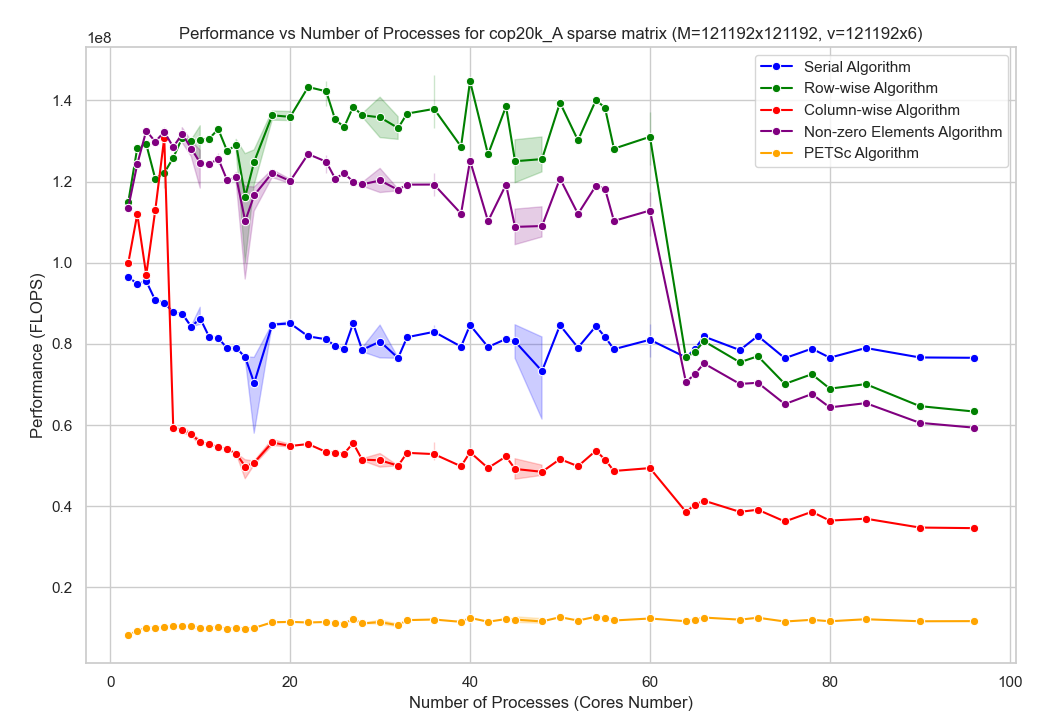
\includegraphics[width=0.5\textwidth]{../results/fat_vector_dim/cop20k_A_k6_performance.png}
    \caption{Cop20k\_A matrix performance}\label{fig:cop20k-a-k6-performance}
\end{figure}

\begin{figure}[H]
    \centering
    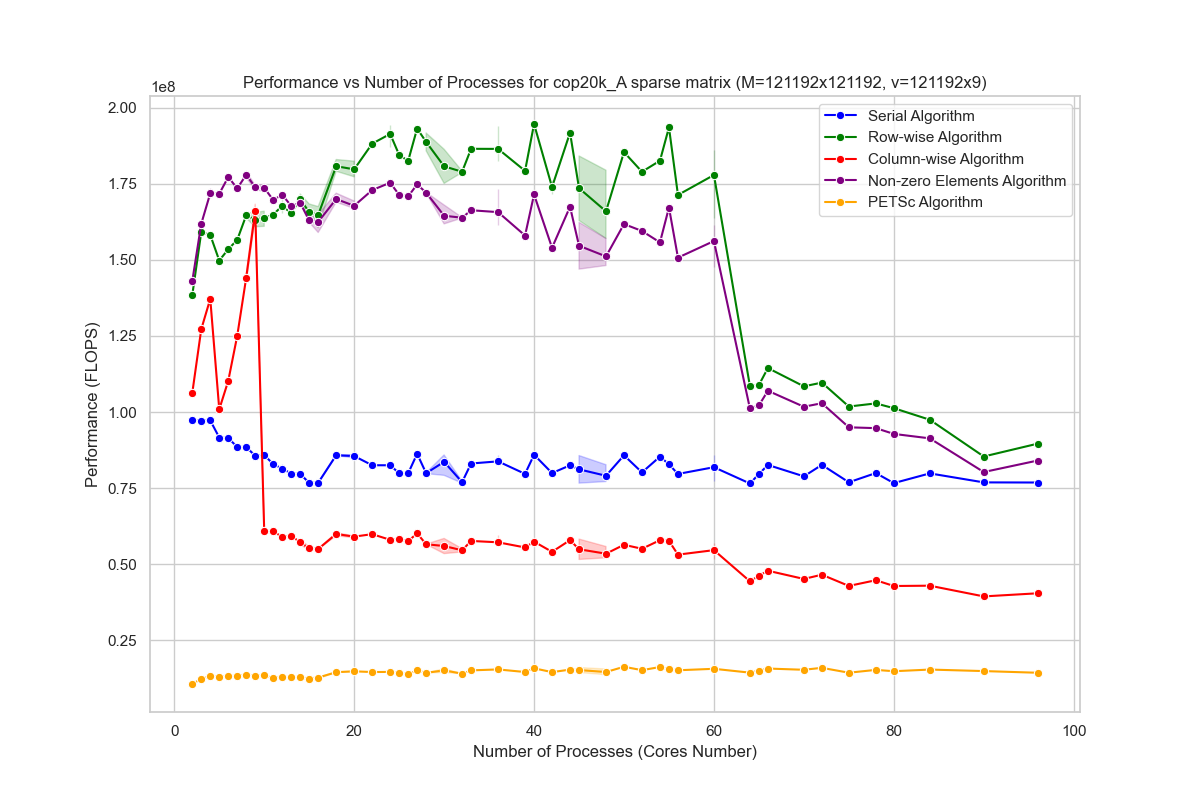
\includegraphics[width=0.5\textwidth]{../results/fat_vector_dim/cop20k_A_k9_performance.png}
    \caption{Cop20k\_A matrix performance}\label{fig:cop20k-a-k9-performance}
\end{figure}

\begin{figure}[H]
    \centering
    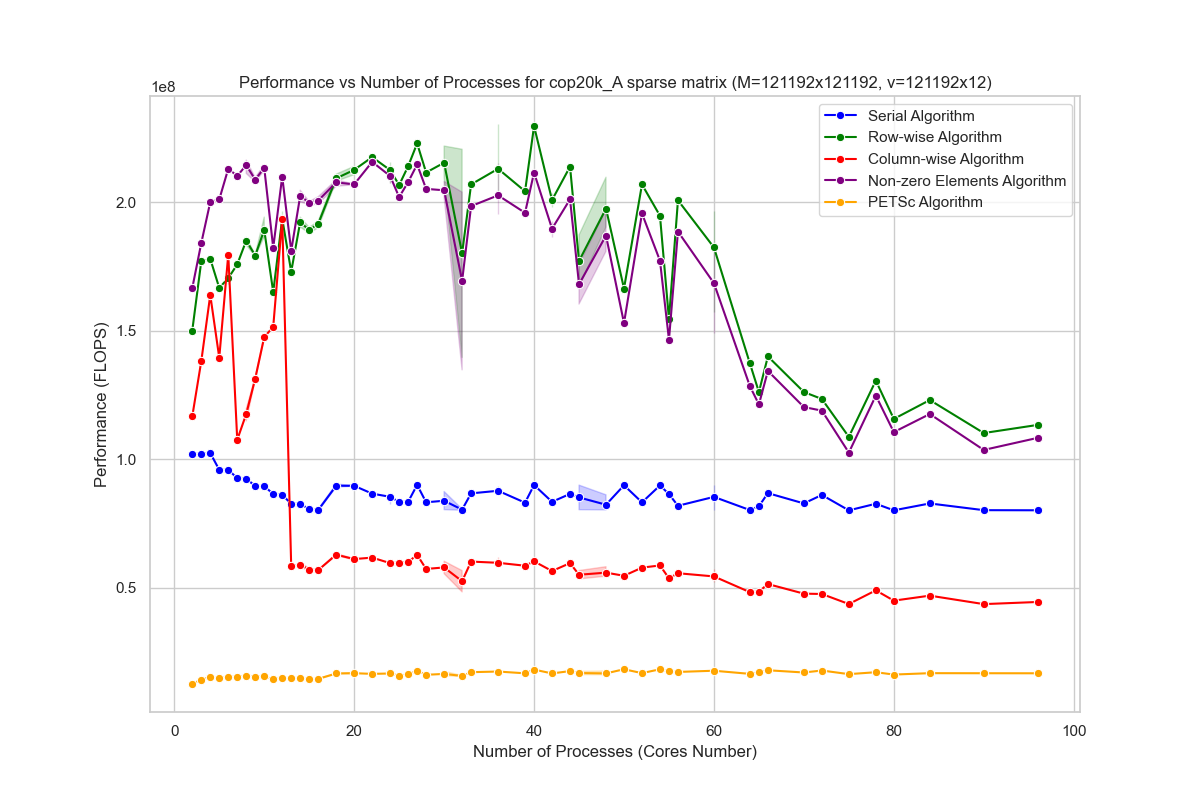
\includegraphics[width=0.5\textwidth]{../results/fat_vector_dim/cop20k_A_k12_performance.png}
    \caption{Cop20k\_A matrix performance}\label{fig:cop20k-a-k12-performance}
\end{figure}

\section{HPC Environmental Impact}
The LUMI supercomputer, based at the CSC-IT Center for Science in Finland,
represents a milestone in the field of high-performance computing (HPC), not
only because of its computing power, but also because of its approach to
environmental sustainability. LUMI, one of EuroHPC's world-class
supercomputers, began operating in 2021 and is expected to reach full capacity
in 2023. It features an environmentally-friendly design and is considered to be
one of the most energy-efficient data centres in the world.

Irina Kupiainen, who works as Programme Director for the Open Scholarship
Innovation Program at the CSC, plays an important role in the development of
policies relating to high-performance computing and open science. With a strong
background in international policy and experience in various government and
research organisations, Irina Kupiainen leads EU public affairs at the CSC,
focusing on policy and international collaboration, particularly in the area of
open science.

The impact of supercomputing on the environment is a major concern, not least
because of the high energy demands of these systems. However, LUMI is an
example of how HPC can make a positive contribution to environmental
sustainability. It runs on 100\% renewable energy and makes efficient use of
waste heat, which can heat up to 20\% of the homes in the surrounding city.
This approach not only reduces the carbon footprint, but also demonstrates
HPC's potential to meet climate neutrality targets.

Furthermore, sustainability measures in HPC are not limited to energy
consumption and waste heat management. The entire life cycle of the machine
needs to be taken into account, including construction, modularity,
scalability, recycling and reuse of materials. This holistic view can
contribute to the development of a circular economy, supporting sustainability
to its full potential.

In conclusion, the LUMI supercomputer, led by experts such as Irina Kupiainen
and others at the CSC-IT Center for Science, illustrates how supercomputing can
be both a powerful tool for scientific progress and a leader in environmental
sustainability. By harnessing renewable energy sources, making efficient use of
waste heat and taking into account the full lifecycle of HPC systems, LUMI is
setting a precedent for how high-performance computing can contribute to a
greener, more sustainable future.

\chapter{Conclusion}

\bibliographystyle{CranfieldNumbered}
\bibliography{CUCitations}

\appendix
\chapter{Documentation}

\begin{subappendices}
    \section{Project tree}
    \begin{lstlisting}[breaklines=true, basicstyle=\small]
    Source Code/
        scripts/
            batch_test.sh
            get_csv_all.sh
            get_csv_debug.sh
            get_csv_specific.sh
            mpi.sub
        MatrixDefinitions.h
        SparseMatrixFatVectorMultiply.h
        SparseMatrixFatVectorMultiply.cpp
        SparseMatrixFatVectorMultiplyRowWise.h
        SparseMatrixFatVectorMultiplyRowWise.cpp
        SparseMatrixFatVectorMultiplyColumnWise.h
        SparseMatrixFatVectorMultiplyColumnWise.cpp
        SparseMatrixFatVectorMultiplyNonZeroElement.h
        SparseMatrixFatVectorMultiplyNonZeroElement.cpp
        utils.h
        utils.cpp
        main.cpp
    results/
        fat_vector_dim/
            <sparse_matrix>_<k>_<metric>.png
        matrix_dim/
            <sparse_matrix>_<k>_<metric>.png
    \end{lstlisting}

    \section{Getting Started}
    To run the program, follow these steps:
    \begin{enumerate}
        \itemindent=17.87pt
        \item Install the required libraries:
              \href{https://docs.open-mpi.org/en/main/installing-open-mpi/quickstart.html}{mpi}
              \& \href{https://petsc.org/release/install/}{petsc}
        \item Compile the main program using the following command:
              \begin{lstlisting}[style=bashstyle]
                mmpicxx -o <executable_name> -I${PETSC_DIR}/include -I${PETSC_DIR}/${PETSC_ARCH}/include -L${PETSC_DIR}/${PETSC_ARCH}/lib -lpetsc SparseMatrixFatVectorMultiply.cpp  main_verify.cpp utils.cpp SparseMatrixFatVectorMultiplyColumnWise.cpp SparseMatrixFatVectorMultiplyNonZeroElement.cpp SparseMatrixFatVectorMultiplyRowWise.cpp
            \end{lstlisting}
        \item Run the program using the following command:
              \begin{lstlisting}[style=bashstyle]
                mpirun -np <number_of_processes> <executable_name> <k> <sparse_matrix_file_pathw>
            \end{lstlisting}
    \end{enumerate}

    \section{Methods Overview}
    \subsection{Utils.h}
    \subsubsection{ConvertPETScMatToFatVector}

    \textbf{Description:} Converts a PETSc matrix to a FatVector stucture.\\

    \textbf{Parameters:}
    \begin{itemize}
        \item \texttt{Mat C} - PETSc matrix to be converted.
    \end{itemize}

    \textbf{Returns:} \texttt{FatVector} - Fat vector representation of the PETSc matrix.

    \subsubsection{areMatricesEqual}
    \textbf{Description:} Compares two matrices for equality within a specified tolerance.\\

    \textbf{Parameters:}
    \begin{itemize}
        \item \texttt{FatVector \&mat1} - First matrix.
        \item \texttt{FatVector \&mat2} - Second matrix.
        \item \texttt{double tolerance} - Tolerance for comparison.
    \end{itemize}

    \textbf{Returns:} \texttt{bool} - True if matrices are equal within the tolerance, false otherwise.

    \subsubsection{readMatrixMarketFile}
    \textbf{Description:} Reads a matrix from a Matrix Market file into a sparse matrix format.\\

    \textbf{Parameters:}
    \begin{itemize}
        \item \texttt{std::string \&filename} - Name of the Matrix Market file.
    \end{itemize}
    
    \textbf{Returns:} \texttt{SparseMatrix} - Sparse matrix read from the file.

    \subsubsection{generateLargeFatVector}
    \textbf{Description:} Generates a random Fat Vector with specified dimensions.\\

    \textbf{Parameters:}
    \begin{itemize}
        \item \texttt{int n} - Number of rows.
        \item \texttt{int k} - Number of columns.
    \end{itemize}

    \textbf{Returns:} \texttt{FatVector} - Generated fat vector.

    \subsubsection{serialize and deserialize}
    \textbf{Description:} Serializes and deserializes a FatVector to and from a flat array, respectively.\\

    \textbf{Parameters for serialize:}
    \begin{itemize}
        \item \texttt{FatVector \&denseVec} - fat vector to serialize.
    \end{itemize}

    \textbf{Returns:} \texttt{std::vector<double>} - Flat array containing the serialized data.\\

    \textbf{Parameters for deserialize:}
    \begin{itemize}
        \item \texttt{std::vector<double> \&flat} - Flat array to deserialize.
        \item \texttt{int rows} - Number of rows in the fat vector.
        \item \texttt{int cols} - Number of columns in the fat vector.
    \end{itemize}

    \textbf{Returns:} \texttt{FatVector} - Deserialized fat vector.

    \subsection{SparseMatrixFatVectorMultiply.h}
    \subsubsection{sparseMatrixFatVectorMultiply}
    \textbf{Description:} Executes the multiplication using a sequential algorithm.\\

    \textbf{Parameters:}
    \begin{itemize}
        \item \texttt{SparseMatrix \&sparseMatrix} - The sparse matrix.
        \item \texttt{FatVector \&fatVector} - The Fat Vector.
        \item \texttt{int vecCols} - Number of columns in the Fat Vector.
    \end{itemize}

    \textbf{Returns:} \texttt{FatVector} - Result of the multiplication.

    \subsection{SparseMatrixFatVectorMultiplyRowWise.h}
    \subsubsection{sparseMatrixFatVectorMultiplyRowWise}
    \textbf{Description:} Multiplies a sparse matrix with a Fat Vector using row-wise distribution.\\

    \textbf{Parameters:}
    \begin{itemize}
        \item \texttt{SparseMatrix \&sparseMatrix} - The sparse matrix.
        \item \texttt{FatVector \&fatVector} - The Fat Vector.
        \item \texttt{int vecCols} - Number of columns in the Fat Vector.
    \end{itemize}

    \textbf{Returns:} \texttt{FatVector} - Result of the multiplication.

    \subsection{SparseMatrixFatVectorMultiplyColumnWise.h}
    \subsubsection{sparseMatrixFatVectorMultiplyColumnWise}
    \textbf{Description:} Executes the multiplication using column-wise parallel algorithm.\\

    \textbf{Parameters:}
    \begin{itemize}
        \item \texttt{SparseMatrix \&sparseMatrix} - The sparse matrix.
        \item \texttt{FatVector \&fatVector} - The Fat Vector.
        \item \texttt{int vecCols} - Number of columns in the Fat Vector.
    \end{itemize}

    \textbf{Returns:} \texttt{FatVector} - Result of the multiplication.

    \subsection{SparseMatrixFatVectorMultiplyNonZeroElement.h}
    \subsubsection{sparseMatrixFatVectorMultiplyNonZeroElement}
    \textbf{Description:} Executes the multiplication using non-zero element parallel algorithm.\\

    \textbf{Parameters:}
    \begin{itemize}
        \item \texttt{SparseMatrix \&sparseMatrix} - The sparse matrix.
        \item \texttt{FatVector \&fatVector} - The Fat Vector.
        \item \texttt{int vecCols} - Number of columns in the Fat Vector.
    \end{itemize}

    \textbf{Returns:} \texttt{FatVector} - Result of the multiplication.

\end{subappendices}

\chapter{Source Codes}
\begin{subappendices}
    \section{Data Structures}\label{appendix:data-structures}
    Data stuctures of the sparse matrix and fat vector.
    \lstinputlisting[style=cstyle]{../Source Code/MatrixDefinitions.h}

    \newpage

    \section{Sequential Algorithm}\label{appendix:sequential}
    Sequential algorithm for multiplying a sparse matrix by a fat vector.
    \subsection{Declaration File}
    \lstinputlisting[style=cstyle]{../Source Code/SparseMatrixFatVectorMultiply.h}
    \subsection{Implementation File}
    \lstinputlisting[style=cstyle]{../Source Code/SparseMatrixFatVectorMultiply.cpp}

    \section{Line-Based Parallelism}\label{appendix:line-based}
    Parallel algorithm for multiplying a sparse matrix by a fat vector using
    line-based parallelism.
    \subsection{Declaration File}
    \lstinputlisting[style=cstyle]{../Source Code/SparseMatrixFatVectorMultiplyRowWise.h}
    \subsection{Implementation File}
    \lstinputlisting[style=cstyle]{../Source Code/SparseMatrixFatVectorMultiplyRowWise.cpp}

    \section{Column-Wise Parallelism}\label{appendix:column-based}
    Parallel algorithm for multiplying a sparse matrix by a fat vector using
    column-wise parallelism.
    \subsection{Declaration File}
    \lstinputlisting[style=cstyle]{../Source Code/SparseMatrixFatVectorMultiplyColumnWise.h}
    \subsection{Implementation File}
    \lstinputlisting[style=cstyle]{../Source Code/SparseMatrixFatVectorMultiplyColumnWise.cpp}

    \section{Non-Zero Element Parallelism}\label{appendix:non-zero}
    Parallel algorithm for multiplying a sparse matrix by a fat vector using
    non-zero element parallelism.
    \subsection{Declaration File}
    \lstinputlisting[style=cstyle]{../Source Code/SparseMatrixFatVectorMultiplyNonZeroElement.h}
    \subsection{Implementation File}
    \lstinputlisting[style=cstyle]{../Source Code/SparseMatrixFatVectorMultiplyNonZeroElement.cpp}

    \section{Utility Functions}\label{appendix:utility}
    Utility functions used by the main file.
    \subsection{Declaration File}
    \lstinputlisting[style=cstyle]{../Source Code/utils.h}
    \subsection{Implementation File}
    \lstinputlisting[style=cstyle]{../Source Code/utils.cpp}

    \section{Main File}\label{appendix:main}
    Main file for running the different algorithms and comparing their performance.
    \lstinputlisting[style=cstyle]{../Source Code/main.cpp}

    \section{Scripts}
    \subsection{MPI Submission Script} \label{appendix:mpi-sub}
    Bash script to submit an MPI job to the cluster.
    \lstinputlisting[style=bashstyle]{../Source Code/scripts/mpi.sub}

    \newpage
    \subsection{Batch Test Script}\label{appendix:batch-test}
    Bash script to submit multiple MPI jobs to the cluster.
    \lstinputlisting[style=bashstyle]{../Source Code/scripts/batch_test.sh}

    \newpage
    \subsection{Get CSV Script}\label{appendix:get-csv}
    Bash script to analyse all job results files and extract the relevant
    information to create a CSV file. \lstinputlisting[style=bashstyle]{../Source
        Code/scripts/get_csv_all.sh}

\end{subappendices}

\end{document}

